\documentclass[UTF8,a4paper,12pt]{ctexart}

% =========================
% 基础宏包
% =========================
\usepackage{geometry}
\usepackage{setspace}
\usepackage{graphicx}
\usepackage{float}
\usepackage{booktabs}
\usepackage{array}
\usepackage{longtable}
\usepackage{tabularx}
\usepackage{multirow}
\usepackage{enumitem}
\usepackage{xcolor}
\usepackage{listings}
\usepackage{hyperref}
\usepackage{caption}
\usepackage{subcaption}
\usepackage{amsmath}
\usepackage{amssymb}

% =========================
% 页面设置
% =========================
\geometry{
    left=2.8cm,
    right=2.8cm,
    top=2.6cm,
    bottom=2.6cm
}

\setstretch{1.35}

% =========================
% 超链接设置
% =========================
\hypersetup{
    colorlinks=true,
    linkcolor=black,
    urlcolor=blue,
    citecolor=black
}

% =========================
% 代码块设置
% =========================
\lstdefinelanguage{Rust}{
    keywords={fn,let,mut,if,else,while,for,in,loop,break,continue,return,match,enum,struct,impl,trait,mod,use,pub,crate,super,Self,self,as,ref},
    sensitive=true,
    morecomment=[l]{//},
    morecomment=[s]{/*}{*/},
    morestring=[b]", 
}

\lstdefinestyle{codeStyle}{
    basicstyle=\ttfamily\fontsize{8.5pt}{9.5pt}\selectfont,
    numbers=left,
    numberstyle=\tiny,
    stepnumber=1,
    numbersep=8pt,
    frame=single,
    breaklines=true,
    tabsize=4,
    showstringspaces=false,
    keywordstyle=\color{blue},
    commentstyle=\color{gray},
    stringstyle=\color{teal}
}

\lstset{style=codeStyle}

% =========================
% 表格列格式
% =========================
\newcolumntype{Y}{>{\raggedright\arraybackslash}X}

% =========================
% 文档信息
% =========================
\title{
    \heiti 编译原理课程大作业报告提纲\\
    \Large 类 Rust 语言词法分析与语法分析工具设计与实现
}

\author{
    学院：\underline{计算机科学与技术学院} \\
    专业：\underline{计算机科学与技术} \\
    小组成员：\underline{白佳煜、胡桥健、庄子硕} \\
    学号：\underline{2352733、2351295、2350998} \\
    指导教师：\underline{卫志华、高珍}
}

\date{\today}

\begin{document}

% =========================
% 封面
% =========================
\maketitle
\thispagestyle{empty}

\newpage

% =========================
% 目录
% =========================
\tableofcontents

\newpage

% =========================
% 正文
% =========================

\section{实验背景与任务要求}

\subsection{实验背景}

编译器前端通常包括词法分析、语法分析和语义分析等阶段。其中，词法分析负责将源程序的字符序列转换为具有明确类别的 token 序列；语法分析则在 token 序列的基础上，根据语言文法识别程序结构，并构造抽象语法树。二者共同构成理解源程序结构的基础，也是后续语义检查、中间代码生成和优化工作的前提。

本次课程大作业以类 Rust 语言为对象，要求实现一个能够进行词法分析和语法分析的编译前端原型。Rust 语言具有较为清晰的语法结构，同时包含函数声明、变量绑定、可变性标记、表达式、控制流、引用、数组和元组等语言特性，因此适合作为编译原理实验中的分析对象。通过实现类 Rust 语言的词法分析器和语法分析器，可以将课堂中关于正规文法、有限自动机、上下文无关文法、语法树和递归下降分析等理论知识落实到具体程序中。

本项目的核心任务并不是实现完整的 Rust 编译器，而是在课程给定的类 Rust 语法范围内，完成从源代码输入到 token 序列输出、再到 AST 构造与展示的基本流程。项目最终应能够接收一段类 Rust 源程序，识别其中的词法单元，判断其是否符合基本语法规则，并以命令行或 Web 页面形式展示分析结果。

\subsection{任务目标}

结合课程要求和本项目的实际实现，本实验的目标可以概括为以下三个层次。

首先，在词法分析层面，需要设计一套能够覆盖类 Rust 词法规则的 token 类型体系，并实现相应的扫描逻辑。词法分析器应能够识别关键字、标识符、整数、运算符、界符、分隔符、特殊符号、注释和结束符等基本词法单元。同时，词法分析器还需要正确处理关键字与标识符之间的边界问题，例如 \texttt{if123} 应被识别为一个标识符，而 \texttt{if=123} 应被拆分为关键字 \texttt{if}、赋值号 \texttt{=} 和整数 \texttt{123}。

其次，在语法分析层面，需要根据课程给定的类 Rust 语法规则，实现对程序结构的识别与抽象语法树构造。语法分析器至少应支持函数声明、形参列表、返回语句、变量声明、赋值语句、基础表达式、比较运算、加减乘除运算、函数调用、if 选择结构和 while 循环结构等核心语法。由于这些结构基本覆盖了一个小型命令式语言的主要组成部分，因此它们也是本项目语法分析器设计的重点。

最后，在工程展示层面，项目需要提供清晰的分析结果输出方式。除命令行运行外，本项目还实现了本地 Web 页面，用于展示 token 表、AST 树和错误信息。这样既便于调试，也便于演示时直观展示词法分析和语法分析的过程与结果。

\subsection{任务范围与实现边界}

需要说明的是，本次大作业的重点在于词法分析和语法分析，而不是完整的语义分析。因此，本项目主要判断源程序在词法和语法层面是否符合规则，并构造相应的 AST；对于变量是否已经声明、赋值类型是否匹配、不可变变量是否被重新赋值、函数返回类型是否一致等问题，目前只在有限范围内处理，尚未形成完整的语义检查体系。

在最低要求之外，本项目还对部分类 Rust 扩展语法进行了支持，例如 \texttt{else}、\texttt{else if}、\texttt{for}、\texttt{loop}、\texttt{break}、\texttt{continue}、引用、数组、元组和表达式块等。这些扩展内容能够增强分析器对类 Rust 程序的覆盖能力，但其语义正确性检查并非本阶段的重点。

因此，本文后续将围绕以下问题展开：

\begin{enumerate}[label=\arabic*.]
    \item 如何设计词法单元类型，并实现对类 Rust 源程序的逐字符扫描；
    \item 如何处理关键字边界、最长匹配、注释跳过和错误定位等词法分析问题；
    \item 如何设计 AST 节点结构，使其能够表达函数、语句、表达式和类型等语法结构；
    \item 如何使用递归下降方法实现语法分析，并正确处理表达式优先级；
    \item 如何通过测试样例和 Web 页面验证分析器的正确性与可展示性。
\end{enumerate}

\section{系统总体设计}

\subsection{总体设计思路}

本项目面向类 Rust 语言的词法分析与语法分析任务，整体设计遵循编译器前端的基本处理流程：首先由词法分析器将源程序字符流转换为 token 序列，然后由语法分析器根据语法规则对 token 序列进行结构化分析，并构造抽象语法树，最后通过命令行或 Web 页面将分析结果展示给用户。

从系统职责上看，本项目并不试图实现完整的 Rust 编译器，而是聚焦于编译前端中最基础、最核心的两个阶段：词法分析和语法分析。词法分析阶段关注“源代码中有哪些词法单元”，语法分析阶段关注“这些词法单元能否组成合法的程序结构”。因此，系统总体设计的核心目标是建立一条清晰的分析流水线，使源程序能够依次经过输入、词法扫描、token 输出、语法解析、AST 构造和结果展示等步骤。

项目采用模块化设计，将词法分析、语法分析和结果展示分别封装为相对独立的模块。这样做的优点是各模块职责清晰，便于分别开发、测试和调试：词法分析器可以独立验证 token 识别是否正确；语法分析器可以在 token 流基础上独立验证 AST 构造是否正确；Web 展示模块则主要负责用户交互和结果可视化，而不直接承担词法或语法规则的实现。

本项目的总体处理流程如图 \ref{fig:system-overview} 所示。

\begin{figure}[H]
    \centering
    \includegraphics[width=1\textwidth]{figures/system-overview.png}
    \caption{系统总体处理流程}
    \label{fig:system-overview}
\end{figure}

\subsection{系统模块划分}

根据功能职责，本项目主要划分为三个核心模块：词法分析模块、语法分析模块和 Web 展示模块。整体结构上，三个核心模块分别对应独立的 Rust crate，便于分别构建和测试。

\begin{table}[H]
    \centering
    \caption{系统核心模块划分}
    \label{tab:module-design}
    \begin{tabularx}{\textwidth}{c|Y|Y}
        \toprule
        模块名称 & 主要职责 & 输出结果 \\
        \midrule
        \texttt{Easy\_Lexer}
        & 读取类 Rust 源代码，完成关键字、标识符、整数、运算符、界符、分隔符、注释等词法单元的识别，并记录 token 的行列位置信息
        & Token 序列和词法错误信息 \\
        \midrule
        \texttt{Easy\_Parser}
        & 调用词法分析器获取 token 流，使用递归下降方法进行语法分析，识别函数、语句、表达式、控制流等语法结构
        & 抽象语法树 AST 和语法错误信息 \\
        \midrule
        \texttt{Easy\_Server}
        & 提供本地 Web 服务和分析接口，将词法分析、语法分析结果返回前端页面进行展示
        & Token 表、AST 树和错误信息的可视化结果 \\
        \bottomrule
    \end{tabularx}
\end{table}

这种模块划分方式与编译器前端的自然阶段相对应。词法分析器只负责将字符流转换为 token，不直接判断复杂语法结构；语法分析器以 token 流为输入，负责识别程序层次结构；Web 服务则作为展示层，将底层分析能力包装为可交互界面。通过这种设计，系统既能满足命令行运行和自动化测试的需要，也能可视化演示及使用的需要，提高了系统的可用性和可维护性。

\subsection{数据流设计}

本项目的数据流围绕“源代码到 AST”的转换过程展开。用户输入的类 Rust 源代码首先以字符串形式进入系统，然后经过词法分析器转换为 token 序列。token 序列保留了源程序中的词法信息，包括 token 类别、原始文本、行号和列号。语法分析器在 token 序列基础上进行递归下降分析，并构造程序的抽象语法树。最后，AST 和错误信息会被序列化为适合输出或展示的形式。

系统的数据流可以分为以下几个阶段：

\begin{enumerate}[label=\arabic*.]
    \item \textbf{源代码输入阶段}：用户通过命令行参数、标准输入或 Web 页面输入类 Rust 源程序；
    \item \textbf{词法扫描阶段}：词法分析器逐字符扫描源代码，生成 token 序列，并记录可能出现的词法错误；
    \item \textbf{语法解析阶段}：语法分析器读取 token 序列，根据文法规则识别函数、语句、表达式和类型等结构；
    \item \textbf{AST 构造阶段}：语法分析器将识别到的语法结构组织为抽象语法树；
    \item \textbf{结果输出阶段}：系统将 token、AST 和错误信息输出到命令行、JSON 文件或 Web 页面。
\end{enumerate}

结合具体代码实现，其数据流关系如图 \ref{fig:data-flow} 所示。

\begin{figure}[H]
    \centering
    \includegraphics[width=0.9\textwidth]{figures/dataflow.png}
    \caption{系统数据流示意图}
    \label{fig:data-flow}
\end{figure}

\section{词法分析器设计与实现}

\subsection{词法分析器的功能定位}

词法分析是编译器前端的第一个阶段，其主要任务是将源程序的字符流转换为具有明确类别的 token 序列。对于后续语法分析器而言，词法分析器起到了屏蔽字符细节、抽象源程序结构的作用。语法分析器不再直接处理单个字符，而是基于词法分析器输出的 token 序列识别更高层次的语法结构。

本项目中的词法分析器位于 \texttt{Easy\_Lexer} 模块中，核心实现文件为 \texttt{lib.rs}。该模块面向课程要求中的类 Rust 语言词法规则，能够识别关键字、标识符、整数、赋值号、算术运算符、比较运算符、界符、分隔符、特殊符号、注释和结束符等词法单元。同时，词法分析器还会为每个 token 记录其在源程序中的行号和列号，以便在后续语法分析或错误提示中定位问题。

从输入输出关系上看，词法分析器的输入是一段 \texttt{\&str} 类型的源代码字符串，输出是一个 \texttt{LexResult} 结构。该结构中包含两个部分：一是扫描得到的 token 列表，二是扫描过程中发现的词法错误列表。这样的设计使得词法分析器不仅能够返回正常分析结果，也能够在出现词法错误时保留错误信息，便于前端页面或命令行程序统一展示。

\subsection{词法分析状态转换图}

词法分析器采用逐字符扫描方式。扫描器从初始状态开始，根据当前字符类别进入不同识别状态，包括标识符或关键字识别状态、整数识别状态、复合符号识别状态、注释处理状态和错误处理状态。每当识别出一个完整 token 后，扫描器将 token 加入结果序列，并重新回到初始状态继续扫描后续字符。

词法分析器的状态转换逻辑可概括为图 \ref{fig:lexer-state-machine} 所示。

\begin{figure}[H]
    \centering
    \includegraphics[width=0.9\textwidth]{figures/lexer-state-machine-detailed.png}
    \caption{词法分析状态转换图}
    \label{fig:lexer-state-machine}
\end{figure}

而对于注释的处理，由如下状态转换图 \ref{fig:comment-state-machine} 所示。

\begin{figure}[H]
    \centering
    \includegraphics[width=0.9\textwidth]{figures/comment-state-machine.png}
    \caption{注释处理状态转换图}
    \label{fig:comment-state-machine}
\end{figure}

\subsection{核心数据结构设计}

\subsubsection{位置信息 Position}

为了支持错误定位和 token 位置展示，词法分析器首先定义了 \texttt{Position} 结构，用于记录某个 token 或词法错误在源程序中的行号和列号。

\begin{lstlisting}[language=Rust,caption={Position 结构定义}]
#[derive(Debug, Clone, Copy, PartialEq, Eq)]
pub struct Position {
    pub line: usize,
    pub column: usize,
}
\end{lstlisting}

其中，\texttt{line} 表示当前 token 所在行，\texttt{column} 表示当前 token 起始位置所在列。词法分析器在扫描过程中会维护当前行列号。当读取普通字符时，列号递增；当读取换行符时，行号递增并将列号重置为 1。通过这种方式，后续一旦发现非法字符、未闭合注释或语法错误，就可以向用户报告较为准确的位置。

\subsubsection{Token 结构}

词法分析器输出的基本单位是 token。本项目中的 token 由三部分组成：token 类别、源程序中的原始文本以及位置信息。

\begin{lstlisting}[language=Rust,caption={Token 结构定义}]
#[derive(Debug, Clone, PartialEq, Eq)]
pub struct Token {
    pub kind: TokenKind,
    pub lexeme: String,
    pub position: Position,
}
\end{lstlisting}

其中，\texttt{kind} 表示 token 的类型，例如关键字、标识符、整数、加号、左括号等；\texttt{lexeme} 保存源程序中的原始字符串，例如 \texttt{"if"}、\texttt{"main"}、\texttt{"123"}；\texttt{position} 则记录该 token 在源程序中的起始位置。

这种设计同时保留了词法类别和源代码文本。词法类别供后续语法分析器判断结构使用，原始文本则便于输出 token 表、生成错误信息或进一步构造 AST 节点。

\subsubsection{TokenKind 枚举}

\texttt{TokenKind} 是词法分析器中最重要的数据结构之一，用于描述所有可识别 token 的类别。本项目将 token 类型划分为关键字、标识符、数字、运算符、界符、分隔符、特殊符号和结束符等几类。

\begin{lstlisting}[language=Rust,caption={TokenKind 枚举定义}]
#[derive(Debug, Clone, PartialEq, Eq)]
pub enum TokenKind {
    Keyword(Keyword),
    Identifier,
    Number,
    Assign,
    Plus,
    ......
}
\end{lstlisting}

其中，关键字并没有被设计为多个独立的 \texttt{TokenKind} 变体，而是统一表示为 \texttt{Keyword(Keyword)}。这种设计将“是否为关键字”和“具体是哪一个关键字”分成两个层次：\texttt{TokenKind} 负责说明该 token 是关键字类别，\texttt{Keyword} 枚举负责说明具体关键字内容。这样可以使 token 类型结构更加清晰，也方便后续语法分析器统一处理关键字。

除关键字外，\texttt{Identifier} 表示标识符，\texttt{Number} 表示整数。运算符部分包括赋值号 \texttt{=}、算术运算符 \texttt{+ - * /}、比较运算符 \texttt{== > >= < <= !=} 和引用相关符号 \texttt{\&}。界符包括圆括号、花括号和方括号；分隔符包括分号、冒号和逗号；特殊符号包括函数返回箭头 \texttt{->}、点号 \texttt{.} 和区间符号 \texttt{..}；\texttt{EndMarker} 则对应课程要求中的结束符 \texttt{\#}。

\subsubsection{Keyword 枚举}

课程要求中给定了一组类 Rust 语言关键字。代码中使用 \texttt{Keyword} 枚举对这些保留字进行统一管理。

\begin{lstlisting}[language=Rust,caption={Keyword 枚举定义}]
#[derive(Debug, Clone, Copy, PartialEq, Eq)]
pub enum Keyword {
    I32,
    Let,
    If,
    Else,
    While,
    Return,
    Mut,
    Fn,
    For,
    In,
    Loop,
    Break,
    Continue,
}
\end{lstlisting}

该枚举覆盖了课程要求中的全部关键字，包括基础类型 \texttt{i32}，变量声明关键字 \texttt{let}，控制流关键字 \texttt{if}、\texttt{else}、\texttt{while}，函数相关关键字 \texttt{fn}、\texttt{return}，可变性关键字 \texttt{mut}，以及扩展语法中使用的 \texttt{for}、\texttt{in}、\texttt{loop}、\texttt{break}、\texttt{continue}。

在实际扫描过程中，词法分析器会先按照标识符规则读取完整单词，然后调用 \texttt{keyword\_from} 函数判断该单词是否属于关键字。如果匹配成功，则生成 \texttt{TokenKind::Keyword(keyword)}；否则生成普通的 \texttt{TokenKind::Identifier}。

\subsubsection{词法错误 LexError 与结果 LexResult}

为了统一表示词法分析结果，代码定义了 \texttt{LexError} 和 \texttt{LexResult} 两个结构。

\begin{lstlisting}[language=Rust,caption={LexError 与 LexResult 结构定义}]
#[derive(Debug, Clone, PartialEq, Eq)]
pub struct LexError {
    pub message: String,
    pub position: Position,
}

#[derive(Debug, Default, Clone, PartialEq, Eq)]
pub struct LexResult {
    pub tokens: Vec<Token>,
    pub errors: Vec<LexError>,
}
\end{lstlisting}

\texttt{LexError} 中包含错误信息和错误位置。例如，当扫描过程中遇到无法识别的字符时，会生成形如 \texttt{unexpected character} 的错误；当块注释未闭合时，会生成 \texttt{unterminated block comment} 错误。

\texttt{LexResult} 同时保存 token 列表和错误列表。这种设计比直接返回 \texttt{Result<Vec<Token>, LexError>} 更适合课程项目中的展示需求。因为词法分析器在遇到某些错误后仍可以继续扫描后续字符，从而一次运行中返回更完整的 token 和错误信息。

\subsection{词法分析器的内部状态设计}

为了完成逐字符扫描，代码内部定义了 \texttt{Lexer} 结构。该结构不对外暴露，而是作为 \texttt{lex} 函数内部使用的扫描器对象。

\begin{lstlisting}[language=Rust,caption={Lexer 内部状态定义}]
struct Lexer<'a> {
    input: &'a str,
    index: usize,
    line: usize,
    column: usize,
    tokens: Vec<Token>,
    errors: Vec<LexError>,
}
\end{lstlisting}

其中，\texttt{input} 保存待扫描的源程序字符串，\texttt{index} 表示当前扫描到的字节位置，\texttt{line} 和 \texttt{column} 表示当前行号和列号，\texttt{tokens} 用于保存已经识别出的 token，\texttt{errors} 用于保存扫描过程中发现的词法错误。

扫描器通过 \texttt{Lexer::new(input)} 初始化。初始状态下，\texttt{index} 为 0，表示从输入字符串开头开始扫描；\texttt{line} 和 \texttt{column} 均为 1，表示源程序第一行第一列；token 列表和错误列表均为空。

这种内部状态设计体现了典型的手写词法分析器结构：扫描器一边读取字符，一边更新当前位置，同时根据识别结果向 token 列表或错误列表中加入信息。

\subsection{公共接口设计}

词法分析器对外提供的主要接口是 \texttt{lex} 函数。

\begin{lstlisting}[language=Rust,caption={词法分析器公共入口函数}]
pub fn lex(input: &str) -> LexResult {
    let mut lexer = Lexer::new(input);
    lexer.lex_all();
    LexResult {
        tokens: lexer.tokens,
        errors: lexer.errors,
    }
}
\end{lstlisting}

该函数接收源代码字符串作为参数，首先创建一个内部 \texttt{Lexer} 对象，然后调用 \texttt{lex\_all} 完成完整扫描，最后将扫描器中的 token 和错误信息封装为 \texttt{LexResult} 返回。

这种接口设计较为简洁。调用方不需要关心词法分析器内部如何维护字符位置、如何读取下一个字符或如何处理注释，只需要调用 \texttt{lex(input)} 即可获得词法分析结果。后续语法分析器、命令行程序和 Web 服务都可以基于该接口复用词法分析能力。

\subsection{主扫描流程设计}

词法分析器的核心扫描逻辑位于 \texttt{lex\_all} 方法中。该方法通过循环不断读取输入字符，直到扫描到输入末尾。

在 \texttt{lex\_all} 中，扫描循环的条件是 \texttt{self.index < self.input.len()}。每轮循环开始时先调用 \texttt{skip\_ignored} 跳过空白字符和注释。如果跳过后已经到达输入末尾，则终止扫描。否则，词法分析器记录当前 token 的起始位置 \texttt{start} 和起始下标 \texttt{start\_index}，随后通过 \texttt{peek} 查看当前字节，并进入对应的识别分支。

\subsection{标识符与关键字识别}

标识符和关键字的识别是词法分析器中的重要部分。代码中使用两个辅助函数定义标识符规则：

\begin{lstlisting}[language=Rust,caption={标识符字符判断函数}]
fn is_identifier_start(byte: u8) -> bool {
    byte.is_ascii_alphabetic() || byte == b'_'
}

fn is_identifier_continue(byte: u8) -> bool {
    is_identifier_start(byte) || byte.is_ascii_digit()
}
\end{lstlisting}

其中，标识符的首字符必须是英文字母或下划线，后续字符可以是英文字母、下划线或数字。这与课程要求中的规则“标识符由字母或下划线开头，后接字母、数字或下划线”一致。

在扫描过程中，如果当前字符满足 \texttt{is\_identifier\_start}，词法分析器会继续读取所有满足 \texttt{is\_identifier\_continue} 的后续字符，形成一个完整的字符串。随后调用 \texttt{keyword\_from} 判断该字符串是否是关键字。

\begin{lstlisting}[language=Rust,caption={关键字匹配函数}]
fn keyword_from(lexeme: &str) -> Option<Keyword> {
    match lexeme {
        "i32" => Some(Keyword::I32),
        "let" => Some(Keyword::Let),
        "if" => Some(Keyword::If),
        "else" => Some(Keyword::Else),
        "while" => Some(Keyword::While),
        "return" => Some(Keyword::Return),
        "mut" => Some(Keyword::Mut),
        "fn" => Some(Keyword::Fn),
        "for" => Some(Keyword::For),
        "in" => Some(Keyword::In),
        "loop" => Some(Keyword::Loop),
        "break" => Some(Keyword::Break),
        "continue" => Some(Keyword::Continue),
        _ => None,
    }
}
\end{lstlisting}

这种处理方式保证了关键字识别具有正确的边界。词法分析器不是看到 \texttt{if} 前缀就立即生成关键字，而是先读取完整单词。例如，对于输入 \texttt{if123}，完整读取结果为 \texttt{"if123"}，该字符串无法在 \texttt{keyword\_from} 中匹配到关键字，因此会被识别为普通标识符。对于输入 \texttt{if=123}，扫描器首先读取到完整单词 \texttt{"if"}，由于后续的 \texttt{=} 不属于标识符字符，因此 \texttt{"if"} 会被匹配为关键字；随后 \texttt{=} 和 \texttt{123} 会分别被识别为赋值号和整数。

这一设计直接满足了课程中对 \texttt{if123} 和 \texttt{if=123} 的特殊测试要求。

\subsection{整数识别}

整数识别逻辑相对直接。当当前字符是 ASCII 数字时，词法分析器进入数字扫描分支。扫描器首先读取当前数字，然后继续读取后续所有连续数字，直到遇到非数字字符为止。最终，该连续数字串会被生成为 \texttt{TokenKind::Number} 类型的 token。

该项目中的数字目前只支持十进制整数形式，尚未支持负数字面量、小数、十六进制数或科学计数法。负号被单独识别为 \texttt{Minus}，因此表达式 \texttt{-1} 在词法层面会被拆分为减号和整数 \texttt{1}，其具体含义需要由语法分析阶段进一步处理。

\subsection{复合 Token 与最长匹配策略}

类 Rust 词法规则中包含若干由两个字符组成的复合符号，例如 \texttt{->}、\texttt{==}、\texttt{>=}、\texttt{<=}、\texttt{!=} 和 \texttt{..}。对于这些符号，词法分析器必须优先进行最长匹配，否则可能会将 \texttt{>=} 错误拆分为 \texttt{>} 和 \texttt{=}，或将 \texttt{..} 错误拆分为两个 \texttt{.}。

代码中使用 \texttt{match\_compound\_token} 方法集中处理复合 token：

\begin{lstlisting}[language=Rust,caption={复合 token 匹配函数}]
fn match_compound_token(&self) -> Option<(TokenKind, usize)> {
    match (self.peek(), self.peek_next()) {
        (Some(b'-'), Some(b'>')) => Some((TokenKind::Arrow, 2)),
        (Some(b'='), Some(b'=')) => Some((TokenKind::EqualEqual, 2)),
        (Some(b'>'), Some(b'=')) => Some((TokenKind::GreaterEqual, 2)),
        (Some(b'<'), Some(b'=')) => Some((TokenKind::LessEqual, 2)),
        (Some(b'!'), Some(b'=')) => Some((TokenKind::NotEqual, 2)),
        (Some(b'.'), Some(b'.')) => Some((TokenKind::DotDot, 2)),
        _ => None,
    }
}
\end{lstlisting}

该函数通过同时查看当前字符和下一个字符来判断是否存在复合 token。如果匹配成功，返回对应的 \texttt{TokenKind} 和 token 宽度。当前实现中的复合 token 宽度均为 2，因此在主扫描逻辑中会连续调用两次 \texttt{advance}，将两个字符一起消费掉，再生成对应 token。

主扫描流程中，复合 token 的识别发生在单字符 token 之前。这一点非常关键。若先识别单字符 token，则 \texttt{==} 会在第一个 \texttt{=} 处被提前识别为 \texttt{Assign}，从而破坏最长匹配原则。当前实现通过先调用 \texttt{match\_compound\_token}，再处理单字符符号，保证了复合符号优先识别。

\subsection{单字符 Token 识别}

当当前字符既不是标识符起始字符，也不是数字，并且不能匹配复合 token 时，词法分析器会尝试将其识别为单字符 token。该部分通过 \texttt{match byte} 实现。

\begin{lstlisting}[language=Rust,caption={单字符 token 识别逻辑}]
let kind = match byte {
    b'=' => Some(TokenKind::Assign),
    b'+' => Some(TokenKind::Plus),
    b'-' => Some(TokenKind::Minus),
    b'*' => Some(TokenKind::Star),
    b'/' => Some(TokenKind::Slash),
    b'>' => Some(TokenKind::Greater),
    b'<' => Some(TokenKind::Less),
    b'&' => Some(TokenKind::Ampersand),
    b'(' => Some(TokenKind::LParen),
    b')' => Some(TokenKind::RParen),
    b'{' => Some(TokenKind::LBrace),
    b'}' => Some(TokenKind::RBrace),
    b'[' => Some(TokenKind::LBracket),
    b']' => Some(TokenKind::RBracket),
    b';' => Some(TokenKind::Semicolon),
    b':' => Some(TokenKind::Colon),
    b',' => Some(TokenKind::Comma),
    b'.' => Some(TokenKind::Dot),
    b'#' => Some(TokenKind::EndMarker),
    _ => None,
};
\end{lstlisting}

这部分覆盖了课程要求中的赋值号、算术运算符、比较运算符中的单字符形式、引用符号、各种括号、分隔符、点号和结束符。若匹配成功，则扫描器调用 \texttt{advance} 消费当前字符，并调用 \texttt{push\_token} 将 token 加入列表。

\subsection{空白字符与注释处理}

源程序中的空白字符和注释不会作为有效 token 传递给语法分析器，因此词法分析器在每轮扫描开始时调用 \texttt{skip\_ignored} 方法跳过这些内容。

\subsubsection{空白字符处理}

当当前字符是 ASCII 空白字符时，词法分析器直接调用 \texttt{advance} 跳过。由于 \texttt{advance} 内部会更新行号和列号，所以即使空白字符不生成 token，也不会影响后续 token 的位置记录。

\subsubsection{单行注释处理}

当词法分析器遇到 \texttt{//} 时，会进入单行注释处理逻辑。扫描器先消费两个斜杠，然后持续读取字符，直到遇到换行符或输入结束为止。单行注释中的内容不会生成 token。

该处理方式符合一般编程语言中单行注释的语义，即从 \texttt{//} 开始到当前行结束之间的内容均被忽略。

\subsubsection{块注释处理}

当词法分析器遇到 \texttt{/*} 时，会进入块注释处理逻辑。代码中不仅支持普通块注释，还通过 \texttt{depth} 变量支持嵌套块注释。扫描器在进入块注释后将 \texttt{depth} 初始化为 1；如果在注释内部再次遇到 \texttt{/*}，则将 \texttt{depth} 加 1；如果遇到 \texttt{*/}，则将 \texttt{depth} 减 1；当 \texttt{depth} 重新变为 0 时，说明最外层块注释已经闭合。

这种设计比只寻找第一个 \texttt{*/} 更健壮。例如，对于如下输入：

\begin{lstlisting}[caption={嵌套块注释示例}]
/* outer /* inner */ outer */
\end{lstlisting}

词法分析器能够正确跳过整个注释，而不会在内部注释结束处提前退出。

如果扫描到输入末尾时 \texttt{depth} 仍未归零，则说明块注释未闭合。此时词法分析器会生成 \texttt{unterminated block comment} 错误，并将错误位置记录为块注释开始的位置。

\subsection{字符读取与位置维护}

词法分析器通过 \texttt{peek}、\texttt{peek\_next}、\texttt{advance} 和 \texttt{position} 等辅助方法完成字符读取和位置维护。

\begin{lstlisting}[language=Rust,caption={字符读取与位置维护函数}]
fn peek(&self) -> Option<u8> {
    self.input.as_bytes().get(self.index).copied()
}

fn peek_next(&self) -> Option<u8> {
    self.input.as_bytes().get(self.index + 1).copied()
}

fn advance(&mut self) -> Option<u8> {
    let byte = self.peek()?;
    self.index += 1;
    if byte == b'\n' {
        self.line += 1;
        self.column = 1;
    } else {
        self.column += 1;
    }
    Some(byte)
}

fn position(&self) -> Position {
    Position {
        line: self.line,
        column: self.column,
    }
}
\end{lstlisting}

其中，\texttt{peek} 用于查看当前字符但不消费，\texttt{peek\_next} 用于查看下一个字符，主要服务于复合 token 和注释识别。\texttt{advance} 用于真正消费当前字符，同时更新 \texttt{index}、\texttt{line} 和 \texttt{column}。\texttt{position} 则用于获取当前扫描位置，通常在识别 token 或记录错误之前调用。

需要注意的是，当前实现以字节为单位扫描，并使用 ASCII 判断函数，例如 \texttt{is\_ascii\_alphabetic} 和 \texttt{is\_ascii\_digit}。这与课程给定的类 Rust 词法规则相匹配，因为课程规则中的字母和数字均限定在 ASCII 范围内。如果后续希望支持 Unicode 标识符，则需要将当前的字节级扫描扩展为字符级扫描。

\subsection{Token 输出与格式化}

当词法分析器成功识别一个 token 后，会调用 \texttt{push\_token} 方法将其加入 token 列表。

\begin{lstlisting}[language=Rust,caption={Token 加入结果列表}]
fn push_token(&mut self, kind: TokenKind, lexeme: &str, position: Position) {
    self.tokens.push(Token {
        kind,
        lexeme: lexeme.to_string(),
        position,
    });
}
\end{lstlisting}

此外，代码还为 \texttt{TokenKind} 和 \texttt{Keyword} 实现了 \texttt{fmt::Display}。这使得 token 类型在命令行输出、测试结果展示或 Web 页面展示时可以转换为更直观的字符串形式。例如，\texttt{TokenKind::Identifier} 会显示为 \texttt{identifier}，\texttt{TokenKind::Keyword(Keyword::If)} 会显示为 \texttt{keyword(if)}。

这种格式化实现虽然不直接影响词法分析的正确性，但能够显著提高结果输出的可读性，有助于实验报告截图展示和调试分析。

\subsection{错误处理机制}

词法分析器的错误处理主要体现在两个方面：非法字符处理和未闭合块注释处理。

当当前字符无法匹配任何合法 token 时，扫描器会将其视为非法字符，并生成一个 \texttt{LexError}：

\begin{lstlisting}[language=Rust,caption={非法字符错误处理}]
let ch = byte as char;
self.errors.push(LexError {
    message: format!("unexpected character `{ch}`"),
    position: start,
});
self.advance();
\end{lstlisting}

这里的设计是“记录错误并继续扫描”。也就是说，词法分析器不会因为遇到一个非法字符就立即终止，而是将错误加入 \texttt{errors} 列表，然后跳过该字符继续处理后续输入。这样可以在一次扫描中尽可能发现更多词法问题。

另一类错误是未闭合块注释。当扫描器进入块注释后，如果直到输入结束都没有找到匹配的结束符 \texttt{*/}，则会生成 \texttt{unterminated block comment} 错误。该错误的位置被设置为块注释开始处，从而方便用户定位问题。

\subsection{词法分析器实现特点}

综合来看，本项目词法分析器具有以下几个实现特点。

第一，数据结构清晰。代码将位置信息、token、token 类型、关键字、错误和最终结果分别定义为独立结构，使词法分析器输出具有较好的可读性和可扩展性。

第二，扫描逻辑直接。词法分析器采用手写逐字符扫描方式，通过 \texttt{peek}、\texttt{peek\_next} 和 \texttt{advance} 控制扫描过程。这种方式实现简单、流程明确，适合课程项目中展示词法分析的基本原理。

第三，关键字识别方式正确。词法分析器先读取完整标识符候选串，再判断其是否为关键字，因此能够正确处理 \texttt{if123} 这类关键字前缀标识符问题。

第四，支持最长匹配。复合 token 的识别被放在单字符 token 之前，保证 \texttt{>=}、\texttt{==}、\texttt{->}、\texttt{..} 等符号不会被错误拆分。

第五，注释处理较完整。词法分析器能够跳过单行注释和块注释，并且块注释部分通过深度计数支持嵌套结构。对于未闭合块注释，也能够给出明确错误信息。

第六，错误处理较友好。词法分析器在遇到非法字符时记录错误并继续扫描，使调用方可以在一次运行中获得更完整的分析结果。

\section{语法分析器设计与实现}

\subsection{语法分析器的功能定位}

语法分析是编译器前端中承接词法分析的重要阶段。词法分析器将源程序字符流转换为 token 序列，而语法分析器则在 token 序列基础上，根据语言文法判断程序结构是否合法，并构造抽象语法树。相比词法分析关注“每个词是什么”，语法分析更关注“这些词如何组成合法的程序”。

本项目中的语法分析器位于 \texttt{Easy\_Parser} 模块中，其输入为 \texttt{Easy\_Lexer} 输出的 token 序列，输出为表示程序结构的抽象语法树。语法分析器能够识别类 Rust 语言中的函数声明、参数列表、返回类型、语句块、变量声明、赋值语句、返回语句、表达式、函数调用、if 选择结构、while 循环等课程强制要求内容。同时，代码还支持 for 循环、loop 循环、break、continue、引用、可变引用、解引用、数组、元组、表达式块、if 表达式和 loop 表达式等扩展结构。

从实现方法上看，本项目采用手写递归下降分析器。递归下降方法的基本思想是：为文法中的主要非终结符设计对应的解析函数，通过函数调用关系体现语法结构。例如，程序由函数声明序列组成，因此 \texttt{parse\_program} 会反复调用 \texttt{parse\_function\_decl}；函数体由语句块组成，因此函数声明解析过程中会继续调用 \texttt{parse\_block}；表达式又按照不同优先级拆分为加减表达式、乘除表达式、一元表达式和基本表达式等层次。这样的设计结构清晰，便于将课程给定的产生式规则映射到代码实现中。

总体来看，本语法分析器的函数调用状态转移图如下所示：
\begin{figure}[H]
    \centering
    \includegraphics[width=0.9\textwidth]{figures/parser-state-machine.png}
    \caption{语法分析状态转换图}
    \label{fig:parser-state-machine}
\end{figure}

\subsection{语法分析器公共接口设计}

语法分析器对外提供了两个主要接口：\texttt{parse\_tokens} 和 \texttt{parse\_program\_ast}。

\begin{lstlisting}[language=Rust,caption={语法分析器公共接口}]
#[allow(dead_code)]
pub fn parse_tokens(tokens: &[Token]) -> Result<(), ParseError> {
    Parser::new(tokens).parse_program().map(|_| ())
}

pub fn parse_program_ast(tokens: &[Token]) -> Result<Program, ParseError> {
    Parser::new(tokens).parse_program()
}
\end{lstlisting}

其中，\texttt{parse\_tokens} 主要用于判断 token 序列是否能够被成功解析。如果解析成功，则返回 \texttt{Ok(())}；如果出现语法错误，则返回 \texttt{ParseError}。该接口适合用于测试语法合法性。

\texttt{parse\_program\_ast} 则返回完整的 \texttt{Program} AST 节点，是本项目中生成语法树的核心接口。命令行工具或 Web 服务可以调用该函数，将词法分析器生成的 token 序列转换为可序列化、可展示的 AST 结构。

这种接口设计将“语法检查”和“AST 生成”进行了区分。前者适合快速判断语法是否正确，后者适合用于后续展示、序列化和进一步分析。

\subsection{语法错误表示}

语法分析过程中可能出现缺少括号、缺少分号、表达式不完整、函数声明格式错误等问题。为了统一描述这些错误，代码定义了 \texttt{ParseError} 结构。

\begin{lstlisting}[language=Rust,caption={ParseError 结构定义}]
#[derive(Debug, Clone, PartialEq, Eq)]
pub struct ParseError {
    pub message: String,
    pub position: Position,
}
\end{lstlisting}

其中，\texttt{message} 表示错误信息，\texttt{position} 表示错误所在位置。该位置直接复用词法分析器中 token 携带的 \texttt{Position}，因此语法错误可以准确定位到源代码中的行号和列号。

代码还为 \texttt{ParseError} 实现了 \texttt{fmt::Display}：

\begin{lstlisting}[language=Rust,caption={ParseError 的显示格式}]
impl fmt::Display for ParseError {
    fn fmt(&self, f: &mut fmt::Formatter<'_>) -> fmt::Result {
        write!(
            f,
            "syntax error at {}:{}: {}",
            self.position.line, self.position.column, self.message
        )
    }
}
\end{lstlisting}

该实现使得错误信息可以以类似 \texttt{syntax error at line:column: message} 的形式输出，便于命令行和 Web 页面展示。相比只提示“语法错误”，这种带位置信息的错误更有助于用户定位源程序中的问题。

\subsection{AST 总体结构设计}

抽象语法树是语法分析器的核心输出。相比具体语法树，AST 会省略一部分语法细节，例如括号、逗号、分号等纯结构性符号，而保留程序真正的层次结构和语义相关信息。本项目中的 AST 节点均支持 \texttt{Serialize}，因此可以方便地转换为 JSON，在命令行或 Web 页面中展示。

从整体上看，本项目的 AST 主要包括以下几类节点：

\begin{itemize}
    \item \texttt{Program}：表示整个程序；
    \item \texttt{FunctionDecl}：表示函数声明；
    \item \texttt{Binding}：表示变量绑定或参数绑定；
    \item \texttt{Block}：表示语句块；
    \item \texttt{Statement}：表示语句；
    \item \texttt{Expr}：表示表达式；
    \item \texttt{TypeNode}：表示类型；
    \item \texttt{UnaryOp} 和 \texttt{BinaryOp}：表示一元和二元运算符；
    \item \texttt{ElseBranch}：表示 if 表达式中的 else 分支。
\end{itemize}

这些节点共同描述了类 Rust 程序的主要结构。顶层 \texttt{Program} 包含若干函数声明；每个函数声明包含函数名、参数列表、返回类型和函数体；函数体是一个 \texttt{Block}，其中包含若干语句和可选的尾表达式；语句和表达式则进一步描述变量声明、赋值、控制流和运算结构。

\subsection{Program 与 FunctionDecl 设计}

程序顶层结构由 \texttt{Program} 表示：

\begin{lstlisting}[language=Rust,caption={Program 节点定义}]
#[derive(Debug, Clone, Serialize)]
pub struct Program {
    pub kind: &'static str,
    pub functions: Vec<FunctionDecl>,
}
\end{lstlisting}

其中，\texttt{kind} 字段用于在 JSON 输出中标识节点类型，\texttt{functions} 保存程序中的函数声明列表。类 Rust 源程序的顶层结构主要由函数声明组成，因此 \texttt{Program} 节点的设计较为直接。

函数声明由 \texttt{FunctionDecl} 表示：

\begin{lstlisting}[language=Rust,caption={FunctionDecl 节点定义}]
#[derive(Debug, Clone, Serialize)]
pub struct FunctionDecl {
    pub kind: &'static str,
    pub name: String,
    pub params: Vec<Binding>,
    #[serde(rename = "returnType")]
    pub return_type: Option<TypeNode>,
    pub body: Block,
}
\end{lstlisting}

其中，\texttt{name} 表示函数名，\texttt{params} 表示参数列表，\texttt{return\_type} 表示可选返回类型，\texttt{body} 表示函数体。返回类型被设计为 \texttt{Option<TypeNode>}，是因为类 Rust 函数既可以显式声明返回类型，例如 \texttt{fn f() -> i32}，也可以没有返回类型，例如 \texttt{fn f()}。

在 JSON 序列化时，代码通过 \texttt{\#[serde(rename = "returnType")]} 将 \texttt{return\_type} 字段重命名为 \texttt{returnType}，使输出结果更适合前端展示。

\subsection{Binding 与类型节点设计}

\subsubsection{Binding 节点}

\texttt{Binding} 用于统一表示函数参数和变量声明中的绑定信息。

\begin{lstlisting}[language=Rust,caption={Binding 节点定义}]
#[derive(Debug, Clone, Serialize)]
pub struct Binding {
    pub kind: &'static str,
    pub mutable: bool,
    pub name: String,
    pub ty: Option<TypeNode>,
}
\end{lstlisting}

其中，\texttt{mutable} 表示是否带有 \texttt{mut} 修饰，\texttt{name} 表示变量名或参数名，\texttt{ty} 表示可选类型标注。将参数和变量声明都抽象为 \texttt{Binding} 有助于复用解析逻辑。例如，函数参数和 let 变量声明都可以通过 \texttt{parse\_binding} 解析，只是在是否必须带类型上有所不同。

\subsubsection{TypeNode 节点}

类型由 \texttt{TypeNode} 枚举表示：

\begin{lstlisting}[language=Rust,caption={TypeNode 节点定义}]
#[derive(Debug, Clone, Serialize)]
#[serde(tag = "kind")]
pub enum TypeNode {
    Named {
        name: String,
    },
    Reference {
        mutable: bool,
        ty: Box<TypeNode>,
    },
    Array {
        element: Box<TypeNode>,
        length: usize,
    },
    Tuple {
        elements: Vec<TypeNode>,
    },
    Unit,
}
\end{lstlisting}

当前实现支持以下类型结构：

\begin{itemize}
    \item \texttt{Named}：命名类型，例如 \texttt{i32}；
    \item \texttt{Reference}：引用类型，例如 \texttt{\&i32} 或 \texttt{\&mut i32}；
    \item \texttt{Array}：数组类型，例如 \texttt{[i32;3]}；
    \item \texttt{Tuple}：元组类型，例如 \texttt{(i32,i32)}；
    \item \texttt{Unit}：空元组类型 \texttt{()}。
\end{itemize}

虽然课程最低要求中只要求支持 \texttt{i32}，但当前实现已经扩展到引用、数组、元组和 unit 类型。需要注意的是，这里的类型节点主要用于语法结构表达，并不代表项目已经实现完整类型检查。变量类型是否匹配、数组元素类型是否一致、函数返回类型是否正确等问题仍属于后续语义分析范围。

\subsection{语句节点设计}

语句由 \texttt{Statement} 枚举表示。代码中使用 \texttt{\#[serde(tag = "kind")]}，使不同语句类型在 JSON 输出中带有明确的 \texttt{kind} 字段。

\begin{lstlisting}[language=Rust,caption={Statement 节点定义}]
#[derive(Debug, Clone, Serialize)]
#[serde(tag = "kind")]
pub enum Statement {
    Empty,
    Let {
        binding: Binding,
        init: Option<Box<Expr>>,
    },
    Assign {
        target: Box<Expr>,
        value: Box<Expr>,
    },
    Expr {
        expr: Box<Expr>,
    },
    Return {
        value: Option<Box<Expr>>,
    },
    While {
        condition: Box<Expr>,
        body: Block,
    },
    For {
        binding: Binding,
        iterable: Box<Expr>,
        body: Block,
    },
    Break {
        value: Option<Box<Expr>>,
    },
    Continue,
}
\end{lstlisting}

该结构覆盖了课程要求中的空语句、变量声明语句、赋值语句、表达式语句、返回语句和 while 循环，也支持扩展语法中的 for 循环、break 和 continue。

其中，\texttt{Let} 语句中的 \texttt{init} 被设计为可选值，因此既能表示 \texttt{let mut a:i32;}，也能表示 \texttt{let mut a:i32=1;}。\texttt{Return} 语句中的 \texttt{value} 也是可选值，因此既能表示 \texttt{return;}，也能表示 \texttt{return expr;}。\texttt{Break} 同样支持可选表达式，从而兼容 loop 表达式中的 \texttt{break value;} 形式。

\subsection{表达式节点设计}

表达式由 \texttt{Expr} 枚举表示（篇幅原因，下面的函数只列出了一部分内容，省略了一些枚举成员）：

\begin{lstlisting}[language=Rust,caption={Expr 节点定义}]
#[derive(Debug, Clone, Serialize)]
#[serde(tag = "kind")]
pub enum Expr {
    Identifier {
        name: String,
    },
    Number {
        value: String,
    },
    Unary {
        op: UnaryOp,
        expr: Box<Expr>,
    }
    ......
}
\end{lstlisting}

该表达式设计覆盖范围较广。其中，\texttt{Identifier} 表示变量名，\texttt{Number} 表示数字字面量，\texttt{Unary} 表示一元表达式，\texttt{Binary} 表示二元表达式，\texttt{Call} 表示函数调用，\texttt{Index} 表示数组索引，\texttt{Field} 表示元组字段访问，\texttt{Array} 和 \texttt{Tuple} 分别表示数组和元组字面量，\texttt{Block}、\texttt{If} 和 \texttt{Loop} 则体现了 Rust 中“块、if、loop 可以作为表达式”的特点。

此外，\texttt{Expr} 还定义了两个辅助方法：

\begin{lstlisting}[language=Rust,caption={表达式辅助判断函数}]
impl Expr {
    fn is_assignable(&self) -> bool {
        match self {
            Self::Identifier { .. } => true,
            Self::Unary {
                op: UnaryOp::Deref, ..
            } => true,
            Self::Index { .. } => true,
            Self::Field { .. } => true,
            _ => false,
        }
    }

    fn can_stand_without_semicolon(&self) -> bool {
        matches!(
            self,
            Self::Block { .. } | Self::If { .. } | Self::Loop { .. }
        )
    }
}
\end{lstlisting}

\texttt{is\_assignable} 用于判断一个表达式是否可以出现在赋值语句左侧。当前实现允许标识符、解引用表达式、数组索引和字段访问作为赋值目标，而不允许数字、二元表达式、函数调用等表达式作为赋值目标。因此，类似 \texttt{1=2;} 的输入会被识别为语法错误。

\texttt{can\_stand\_without\_semicolon} 用于处理块表达式、if 表达式和 loop 表达式。在 Rust 风格语法中，某些表达式结构可以在语句块中不带分号地出现，并作为块的尾表达式或独立表达式处理。该函数为块解析提供了判断依据。

\subsection{Parser 内部状态设计}

语法分析器内部使用 \texttt{Parser} 结构维护 token 序列和当前解析位置。

\begin{lstlisting}[language=Rust,caption={Parser 内部状态定义}]
struct Parser<'a> {
    tokens: &'a [Token],
    current: usize,
}
\end{lstlisting}

其中，\texttt{tokens} 是词法分析器输出的 token 切片，\texttt{current} 表示当前正在查看的 token 下标。语法分析器通过 \texttt{peek\_kind} 查看当前 token 类型，通过 \texttt{advance} 消费当前 token，通过 \texttt{match\_simple}、\texttt{expect\_simple}、\texttt{match\_keyword}、\texttt{expect\_keyword} 等方法实现匹配和错误报告。

这种设计是递归下降分析器的典型实现方式。解析函数之间共享同一个 \texttt{current} 指针，每当成功识别一个 token，就推进指针；如果当前 token 不符合预期，则构造 \texttt{ParseError} 返回。

\subsection{程序与函数声明解析}

\subsubsection{程序解析}

程序解析从 \texttt{parse\_program} 开始。

\begin{lstlisting}[language=Rust,caption={程序解析函数}]
fn parse_program(mut self) -> Result<Program, ParseError> {
    let mut functions = Vec::new();

    while !self.is_at_end() && !self.check_simple(SimpleTokenKind::EndMarker) {
        functions.push(self.parse_function_decl()?);
    }

    if self.match_simple(SimpleTokenKind::EndMarker) && !self.is_at_end() {
        return Err(self.error_here("unexpected tokens after `#`"));
    }

    if !self.is_at_end() {
        return Err(self.error_here("unexpected trailing tokens"));
    }

    Ok(Program::new(functions))
}
\end{lstlisting}

该函数反复解析函数声明，直到 token 流结束或遇到结束符 \texttt{\#}。如果遇到结束符后仍然存在其他 token，则报告 \texttt{unexpected tokens after \#} 错误。该设计支持课程要求中的结束符，同时保证结束符之后不允许再出现额外程序内容。

\subsubsection{函数声明解析}

函数声明由 \texttt{parse\_function\_decl} 解析。

\begin{lstlisting}[language=Rust,caption={函数声明解析函数}]
fn parse_function_decl(&mut self) -> Result<FunctionDecl, ParseError> {
    self.expect_keyword(Keyword::Fn)?;
    let name = self.expect_identifier("expected function name after `fn`")?;
    self.expect_simple(SimpleTokenKind::LParen, "expected `(` after function name")?;
    let params = self.parse_parameter_list()?;
    self.expect_simple(
        SimpleTokenKind::RParen,
        "expected `)` after function parameter list",
    )?;

    let return_type = if self.match_simple(SimpleTokenKind::Arrow) {
        Some(self.parse_type()?)
    } else {
        None
    };

    let body = self.parse_block()?;
    Ok(FunctionDecl::new(name, params, return_type, body))
}
\end{lstlisting}

函数声明解析严格对应类 Rust 函数结构：首先匹配 \texttt{fn} 关键字，然后读取函数名，解析圆括号中的参数列表，再解析可选的返回类型，最后解析函数体语句块。例如：

\begin{lstlisting}[caption={函数声明示例}]
fn base(mut a:i32) -> i32 {
    return a;
}
\end{lstlisting}

该输入会被解析为一个 \texttt{FunctionDecl} 节点，其中函数名为 \texttt{base}，参数列表中包含一个可变参数 \texttt{a:i32}，返回类型为 \texttt{i32}，函数体为一个 \texttt{Block}。

\subsection{参数与变量绑定解析}

参数列表由 \texttt{parse\_parameter\_list} 解析。若当前 token 为右括号，则说明参数列表为空；否则循环解析一个或多个参数绑定，并使用逗号分隔。

\begin{lstlisting}[language=Rust,caption={参数列表解析函数}]
fn parse_parameter_list(&mut self) -> Result<Vec<Binding>, ParseError> {
    let mut params = Vec::new();

    if self.check_simple(SimpleTokenKind::RParen) {
        return Ok(params);
    }

    loop {
        let binding = self.parse_binding(true)?;
        if binding.ty.is_none() {
            return Err(self.error_here("expected `:` after parameter name"));
        }
        params.push(binding);

        if !self.match_simple(SimpleTokenKind::Comma) {
            break;
        }
    }

    Ok(params)
}
\end{lstlisting}

参数绑定和变量绑定共用 \texttt{parse\_binding} 函数。

\begin{lstlisting}[language=Rust,caption={绑定解析函数}]
fn parse_binding(&mut self, require_type: bool) -> Result<Binding, ParseError> {
    let mutable = self.match_keyword(Keyword::Mut);
    let name = self.expect_identifier("expected variable name")?;
    let ty = if self.match_simple(SimpleTokenKind::Colon) {
        Some(self.parse_type()?)
    } else {
        None
    };

    if require_type && ty.is_none() {
        return Err(self.error_here("expected `:` after parameter name"));
    }

    Ok(Binding::new(name, mutable, ty))
}
\end{lstlisting}

该函数首先尝试匹配可选的 \texttt{mut}，然后读取变量名，最后解析可选类型标注。如果 \texttt{require\_type} 为 \texttt{true}，则要求必须带类型。这正好符合函数参数和变量声明之间的差异：函数参数必须写出类型，而 let 变量声明可以在扩展语法中省略类型。

\subsection{类型解析}

类型解析由 \texttt{parse\_type} 完成。该函数支持命名类型、引用类型、数组类型、元组类型和 unit 类型。

\begin{lstlisting}[language=Rust,caption={类型解析函数结构示意}]
fn parse_type(&mut self) -> Result<TypeNode, ParseError> {
    if self.match_keyword(Keyword::I32) {
        return Ok(TypeNode::Named {
            name: "i32".to_string(),
        });
    }

    if self.match_simple(SimpleTokenKind::Ampersand) {
        let mutable = self.match_keyword(Keyword::Mut);
        return Ok(TypeNode::Reference {
            mutable,
            ty: Box::new(self.parse_type()?),
        });
    }

    if self.match_simple(SimpleTokenKind::LBracket) {
        // parse array type: [Type; NUM]
    }

    if self.match_simple(SimpleTokenKind::LParen) {
        // parse tuple type or unit type
    }

    Err(self.error_here("expected a type"))
}
\end{lstlisting}

对于 \texttt{i32}，解析器生成 \texttt{TypeNode::Named}。对于引用类型，解析器先匹配 \texttt{\&}，再判断是否带有 \texttt{mut}，然后递归调用 \texttt{parse\_type} 解析被引用的类型。例如，\texttt{\&mut i32} 会被解析为一个可变引用类型，其内部类型为 \texttt{i32}。

数组类型的形式为：

\begin{lstlisting}[caption={数组类型示例}]
[i32;3]
\end{lstlisting}

解析器会在左方括号后解析元素类型，然后要求出现分号，再读取数组长度数字，最后匹配右方括号。

元组类型的形式为：

\begin{lstlisting}[caption={元组类型示例}]
(i32,i32)
\end{lstlisting}

解析器通过逗号判断其为元组类型。如果圆括号内部为空，即 \texttt{()}，则解析为 \texttt{TypeNode::Unit}。如果元组类型中只有第一个类型而没有逗号，代码会报错，因为元组类型要求第一个元素类型后必须有逗号。

\subsection{语句块与尾表达式解析}

Rust 风格语言中，语句块不仅可以包含若干语句，还可以包含一个不带分号的尾表达式。本项目中的 \texttt{Block} 结构正是为此设计的：

\begin{lstlisting}[language=Rust,caption={Block 节点定义}]
#[derive(Debug, Clone, Serialize)]
pub struct Block {
    pub kind: &'static str,
    pub statements: Vec<Statement>,
    pub tail: Option<Box<Expr>>,
}
\end{lstlisting}

其中，\texttt{statements} 保存普通语句，\texttt{tail} 保存可选尾表达式。例如：

\begin{lstlisting}[caption={带尾表达式的语句块}]
{
    let t = 1;
    t
}
\end{lstlisting}

该块中 \texttt{let t = 1;} 是普通语句，而最后的 \texttt{t} 没有分号，因此会被解析为尾表达式。

语句块解析由 \texttt{parse\_block} 完成。其基本逻辑是：先匹配左花括号，然后不断解析块内部内容，直到遇到右花括号。

这里的设计体现了类 Rust 语法的特点：块内部内容既可能以关键字开头，例如 \texttt{let}、\texttt{return}、\texttt{while}，也可能以表达式开头，例如变量、数字、块表达式或 if 表达式。因此，解析器首先使用 \texttt{starts\_forced\_statement} 判断当前 token 是否必然属于语句开头。如果是，则调用 \texttt{parse\_statement}；否则先尝试解析表达式，再根据后续 token 判断它是赋值语句、表达式语句还是尾表达式。

\subsection{语句解析}

普通语句由 \texttt{parse\_statement} 解析。该函数通过检查当前 token 的类型分派到不同语句分支。
按照空语句、变量声明语句、返回语句、while 循环、for 循环、break 和 continue 的顺序进行检查，最后如果都不匹配，则报告 \texttt{expected a statement} 错误。

\subsubsection{空语句}

当当前 token 为分号时，解析器生成 \texttt{Statement::Empty}。这对应课程规则中的空语句。

\subsubsection{变量声明语句}

当当前 token 为 \texttt{let} 时，解析器调用 \texttt{parse\_binding(false)} 解析变量绑定，然后判断是否存在初始化表达式。如果存在赋值号，则继续解析初始化表达式；最后要求以分号结束。

该设计同时支持以下形式：

\begin{lstlisting}[caption={变量声明语句示例}]
let mut a:i32;
let c=1;
let mut b:i32=2;
\end{lstlisting}

\subsubsection{返回语句}

当当前 token 为 \texttt{return} 时，解析器判断下一个 token 是否为分号。如果是，则解析为无返回值的 \texttt{return;}；否则解析一个返回表达式，并要求最后出现分号。因此当前实现同时支持：

\begin{lstlisting}[caption={返回语句示例}]
return;
return a+1;
\end{lstlisting}

\subsubsection{while 循环}

当当前 token 为 \texttt{while} 时，解析器先解析条件表达式，再解析循环体语句块，最终构造 \texttt{Statement::While} 节点。

\begin{lstlisting}[caption={while 循环示例}]
while a != 0 {
    a = a - 1;
}
\end{lstlisting}

\subsubsection{for 循环}

扩展语法中还支持 \texttt{for} 循环。解析器在匹配 \texttt{for} 后，先解析循环变量绑定，再要求出现 \texttt{in} 关键字，然后解析可迭代表达式和循环体。

\begin{lstlisting}[caption={for 循环示例}]
for mut i in 0..a {
    if i==2 { continue; }
}
\end{lstlisting}

可迭代结构由 \texttt{parse\_iterable} 解析。若表达式后出现 \texttt{..}，则构造 \texttt{BinaryOp::Range} 表达式，用于表示区间。

\subsubsection{break 与 continue}

\texttt{break} 支持可选表达式，因此既可以表示普通循环跳出，也可以用于 loop 表达式返回值：

\begin{lstlisting}[caption={break 和 continue 示例}]
break;
break v;
continue;
\end{lstlisting}

\texttt{continue} 后不允许带表达式，必须直接以分号结束。

\subsection{赋值语句解析与左值检查}

赋值语句并没有在 \texttt{parse\_statement} 中直接作为关键字分支处理，而是在 \texttt{parse\_block} 中通过“先解析表达式，再判断是否跟随赋值号”的方式处理。这是因为赋值语句的开头可能是多种表达式形式，例如：

\begin{lstlisting}[caption={赋值左侧示例}]
a = 1;
*a = 2;
arr[0] = 3;
pair.0 = 4;
\end{lstlisting}

解析器先解析出左侧表达式，如果后面出现赋值号，则判断该表达式是否可赋值：

\begin{lstlisting}[language=Rust,caption={赋值左侧检查逻辑}]
if self.match_simple(SimpleTokenKind::Assign) {
    if !expr.is_assignable() {
        return Err(self.error_here("left side of assignment is not assignable"));
    }
    let value = self.parse_expression()?;
    self.expect_simple(
        SimpleTokenKind::Semicolon,
        "expected `;` after assignment statement",
    )?;
    statements.push(Statement::Assign {
        target: Box::new(expr),
        value: Box::new(value),
    });
    continue;
}
\end{lstlisting}

该设计能够避免非法赋值目标。例如：

\begin{lstlisting}[caption={非法赋值示例}]
1 = 2;
\end{lstlisting}

由于数字表达式不满足 \texttt{is\_assignable}，解析器会报告 \texttt{left side of assignment is not assignable} 错误。这虽然还不是完整语义分析，但已经在语法结构层面对赋值左侧进行了基本限制。

\subsection{表达式解析与优先级处理}

表达式解析是语法分析器中最复杂的部分之一。为了正确处理运算符优先级，本项目将表达式解析拆分为多个层次：

\begin{lstlisting}[language=Rust,caption={表达式解析层次}]
parse_expression()
    -> parse_additive()
        -> parse_multiplicative()
            -> parse_unary()
                -> parse_postfix()
                    -> parse_primary()
\end{lstlisting}

当前实现中，比较运算位于 \texttt{parse\_expression} 层，加减运算位于 \texttt{parse\_additive} 层，乘除运算位于 \texttt{parse\_multiplicative} 层，一元运算位于 \texttt{parse\_unary} 层，函数调用、索引和字段访问等后缀运算位于 \texttt{parse\_postfix} 层，数字、标识符、括号表达式、数组、元组、块、if 和 loop 等基本结构位于 \texttt{parse\_primary} 层。

这种分层设计保证了表达式优先级的正确性。例如，对于表达式：

\begin{lstlisting}[caption={表达式优先级示例}]
a + 1 * 2
\end{lstlisting}

解析器会先在乘除层将 \texttt{1*2} 组合为一个乘法表达式，再在加减层与 \texttt{a} 组合为加法表达式。因此最终 AST 能够正确体现“乘法优先于加法”。

\subsubsection{比较表达式}

比较运算由 \texttt{parse\_expression} 中的循环处理。该函数先解析一个加减表达式，然后不断匹配比较运算符：

\begin{lstlisting}[language=Rust,caption={比较表达式解析}]
fn parse_expression(&mut self) -> Result<Expr, ParseError> {
    let mut expr = self.parse_additive()?;

    while let Some(op) = self.match_comparison_op() {
        let right = self.parse_additive()?;
        expr = Expr::Binary {
            left: Box::new(expr),
            op,
            right: Box::new(right),
        };
    }

    Ok(expr)
}
\end{lstlisting}

比较运算符包括 \texttt{<}、\texttt{<=}、\texttt{>}、\texttt{>=}、\texttt{==} 和 \texttt{!=}。这些运算符统一被转换为 \texttt{BinaryOp} 中的对应枚举值。

\subsubsection{加减表达式}

加减表达式由 \texttt{parse\_additive} 解析。该函数先解析乘除表达式，再循环处理 \texttt{+} 和 \texttt{-}。

这种写法使加减运算天然具有左结合性。例如，\texttt{a-b-c} 会被解析为 \texttt{(a-b)-c}。

\subsubsection{乘除表达式}

乘除表达式由 \texttt{parse\_multiplicative} 解析。该函数与加减表达式类似，但处理的是 \texttt{*} 和 \texttt{/}。由于 \texttt{parse\_additive} 会调用 \texttt{parse\_multiplicative}，因此乘除运算的优先级高于加减运算。

\subsubsection{一元表达式}

一元表达式由 \texttt{parse\_unary} 解析，支持引用、可变引用、解引用和取负操作：

\begin{lstlisting}[caption={一元表达式示例}]
&a
&mut a
*a
-a
\end{lstlisting}

其中，\texttt{\&} 会生成 \texttt{UnaryOp::Ref}，\texttt{\&mut} 会生成 \texttt{UnaryOp::RefMut}，\texttt{*} 会生成 \texttt{UnaryOp::Deref}，\texttt{-} 会生成 \texttt{UnaryOp::Neg}。引用和解引用表达式递归调用 \texttt{parse\_unary}，从而支持连续一元运算。

\subsection{后缀表达式解析}

后缀表达式由 \texttt{parse\_postfix} 处理。该函数先解析一个基本表达式，然后循环判断其后是否跟随函数调用、数组索引或字段访问。

\begin{lstlisting}[language=Rust,caption={后缀表达式解析函数结构示意}]
fn parse_postfix(&mut self) -> Result<Expr, ParseError> {
    let mut expr = self.parse_primary()?;

    loop {
        if self.check_simple(SimpleTokenKind::LParen) && Self::is_callable(&expr) {
            // parse function call
            continue;
        }

        if self.match_simple(SimpleTokenKind::LBracket) {
            // parse array index
            continue;
        }

        if self.match_simple(SimpleTokenKind::Dot) {
            // parse tuple field
            continue;
        }

        break;
    }

    Ok(expr)
}
\end{lstlisting}

该设计使后缀操作可以连续出现。例如，理论上可以解析类似 \texttt{arr[0].1} 这样的链式结构。当前实现中，函数调用要求 callee 必须是标识符、字段访问或索引表达式，这由 \texttt{is\_callable} 函数控制。

数组索引形如：

\begin{lstlisting}[caption={数组索引示例}]
arr[0]
\end{lstlisting}

元组字段访问形如：

\begin{lstlisting}[caption={元组字段访问示例}]
pair.0
\end{lstlisting}

字段访问中，点号后必须是数字文本，这与 Rust 元组字段访问的形式一致。

\subsection{基本表达式解析}

基本表达式由 \texttt{parse\_primary} 解析，是表达式解析的底层入口。该函数支持数字、标识符、块表达式、if 表达式、loop 表达式、数组字面量、元组字面量和括号表达式。

\subsubsection{数字与标识符}

当当前 token 为 \texttt{Number} 时，解析器生成 \texttt{Expr::Number}；当当前 token 为 \texttt{Identifier} 时，生成 \texttt{Expr::Identifier}。

\subsubsection{块表达式}

如果当前 token 为左花括号，解析器直接调用 \texttt{parse\_block}，并将结果包装为 \texttt{Expr::Block}。这体现了 Rust 中块可以作为表达式的特点。

\subsubsection{if 表达式}

当当前 token 为 \texttt{if} 时，解析器调用 \texttt{parse\_if\_after\_keyword} 解析 if 表达式。

\begin{lstlisting}[language=Rust,caption={if 表达式解析函数}]
fn parse_if_after_keyword(&mut self) -> Result<Expr, ParseError> {
    let condition = self.parse_expression()?;
    let then_branch = self.parse_block()?;
    let else_branch = if self.match_keyword(Keyword::Else) {
        if self.match_keyword(Keyword::If) {
            ElseBranch::ElseIf {
                expr: Box::new(self.parse_if_after_keyword()?),
            }
        } else {
            ElseBranch::Block {
                block: self.parse_block()?,
            }
        }
    } else {
        ElseBranch::None
    };

    Ok(Expr::If {
        condition: Box::new(condition),
        then_branch,
        else_branch,
    })
}
\end{lstlisting}

该函数支持无 else 的 if、带 else 的 if，以及链式 else if。需要注意的是，当前实现将 if 统一作为表达式节点处理。当 if 出现在语句块中并带有分号或作为独立结构出现时，会在块解析逻辑中进一步转换为表达式语句或尾表达式。

\subsubsection{loop 表达式}

当当前 token 为 \texttt{loop} 时，解析器将其解析为 \texttt{Expr::Loop}，其内部包含一个语句块。这使得 \texttt{loop} 既可以作为循环结构，也可以作为带 \texttt{break value;} 的表达式结构使用。

\subsubsection{数组字面量}

数组字面量形如：

\begin{lstlisting}[caption={数组字面量示例}]
[1,2,3]
\end{lstlisting}

解析器在遇到左方括号后，调用 \texttt{parse\_expression\_list} 解析表达式列表，直到遇到右方括号为止。

\subsubsection{元组与括号表达式}

圆括号结构需要区分元组表达式和普通括号表达式。当前解析逻辑是：遇到左括号后，先解析第一个表达式；如果后续出现逗号，则认为这是元组表达式；否则认为这是普通括号表达式。

例如：

\begin{lstlisting}[caption={元组表达式与括号表达式示例}]
(1,2)
(1)
()
\end{lstlisting}

其中，\texttt{(1,2)} 被解析为元组表达式，\texttt{(1)} 被解析为普通表达式，\texttt{()} 被解析为空元组表达式。

\subsection{token 匹配辅助机制}

为了简化 token 匹配逻辑，代码中定义了 \texttt{SimpleTokenKind} 枚举，用于表示不含关键字参数的普通 token 类型。

\begin{lstlisting}[language=Rust,caption={SimpleTokenKind 枚举}]
#[derive(Debug, Clone, Copy)]
enum SimpleTokenKind {
    Identifier,
    Number,
    Assign,
    ......
}
\end{lstlisting}

由于 \texttt{TokenKind::Keyword} 中还包含具体关键字，普通 token 和关键字 token 的匹配逻辑有所不同。代码中通过 \texttt{match\_simple} 和 \texttt{match\_keyword} 分别处理普通 token 和关键字 token。

\begin{lstlisting}[language=Rust,caption={普通 token 与关键字匹配函数}]
fn match_simple(&mut self, expected: SimpleTokenKind) -> bool {
    if self.check_simple(expected) {
        self.advance();
        true
    } else {
        false
    }
}

fn match_keyword(&mut self, keyword: Keyword) -> bool {
    if matches!(self.peek_kind(), Some(TokenKind::Keyword(actual)) if *actual == keyword) {
        self.advance();
        true
    } else {
        false
    }
}
\end{lstlisting}

对于必须出现的 token，则使用 \texttt{expect\_simple} 和 \texttt{expect\_keyword}。如果匹配失败，解析器会调用 \texttt{error\_here} 生成带当前位置的错误信息。

\subsection{错误报告机制}

语法错误由 \texttt{error\_here} 函数统一生成。

\begin{lstlisting}[language=Rust,caption={语法错误生成函数}]
fn error_here(&self, message: &str) -> ParseError {
    if let Some(token) = self.tokens.get(self.current) {
        ParseError {
            message: format!("{message}, found `{}`", token.lexeme),
            position: token.position,
        }
    } else if let Some(token) = self.tokens.last() {
        ParseError {
            message: format!("{message}, found end of input"),
            position: token.position,
        }
    } else {
        ParseError {
            message: format!("{message}, found empty input"),
            position: Position { line: 1, column: 1 },
        }
    }
}
\end{lstlisting}

该函数根据当前解析位置生成错误。如果当前 token 存在，则错误信息中会包含实际遇到的 token 文本；如果已经到达输入末尾，则提示 \texttt{found end of input}；如果 token 列表为空，则提示 \texttt{found empty input}。这种设计提高了错误信息的可解释性。

例如，当赋值语句左侧不是合法左值时，解析器会报告 \texttt{left side of assignment is not assignable}。当函数参数缺少类型标注时，会报告 \texttt{expected `:` after parameter name}。当语句块缺少右花括号时，会报告 \texttt{expected `\}` to close the block}。

\subsection{语法分析器实现特点}

综合来看，本项目语法分析器具有以下几个特点。

第一，采用手写递归下降方法，结构清晰。程序、函数、参数、类型、语句块、语句和表达式分别由不同解析函数处理，函数调用关系与语法层次基本对应，便于理解和维护。

第二，AST 设计较完整。节点类型覆盖程序、函数、绑定、块、语句、表达式和类型等主要结构，并支持序列化为 JSON，便于命令行输出和 Web 页面展示。

第三，表达式优先级处理清楚。解析器将比较、加减、乘除、一元、后缀和基本表达式拆分为多个层级，从而正确处理常见表达式的优先级和结合性。

第四，支持较多扩展语法。在最低要求之外，解析器还支持 for、loop、break、continue、引用、数组、元组、表达式块和 if 表达式等结构，使项目对类 Rust 语法具有更好的覆盖能力。

第五，包含基础的赋值左侧检查。虽然当前项目尚未实现完整语义分析，但解析器已经通过 \texttt{is\_assignable} 限制了赋值语句左侧的合法形式，能够识别 \texttt{1=2;} 这类明显非法的赋值结构。

第六，错误信息包含位置和实际 token。借助词法分析器提供的行列号，语法分析器能够在错误信息中指出错误发生位置和实际遇到的 token，有助于调试和展示。

\section{Web 可视化系统设计}

\subsection{设计目标}

为了提升词法分析器和语法分析器的可用性与展示效果，本项目在命令行运行方式之外，额外设计并实现了一个本地 Web 可视化系统。该系统的主要目标不是重新实现词法分析或语法分析逻辑，而是将已经完成的 \texttt{Easy\_Lexer} 和 \texttt{Easy\_Parser} 封装为一个可交互的分析服务，使用户能够在浏览器中输入类 Rust 源程序，并直观查看 token 序列、抽象语法树以及错误信息。

相较于命令行输出，Web 可视化系统具有更好的展示性。词法分析结果可以以表格形式呈现，便于观察每个 token 的类别、文本内容和位置信息；语法分析结果可以以 JSON 或树状结构展示，便于理解源程序被解析后的层次化结构；错误信息也可以集中显示，方便用户快速判断输入程序中存在的词法或语法问题。因此，该模块既有助于开发阶段的调试，也适合课程验收和答辩时进行演示。

从系统定位上看，Web 可视化系统属于展示层和接口层。它不直接承担 token 识别和 AST 构造工作，而是作为前端页面与底层分析器之间的桥梁：前端负责接收用户输入和展示结果，后端负责调用词法分析器、语法分析器并组织返回数据。

\subsection{系统结构}

Web 可视化系统主要由前端页面和后端服务两部分组成。前端页面提供代码输入区域、分析触发按钮和结果展示区域；后端服务负责接收前端提交的源代码，调用词法分析和语法分析模块，并将分析结果封装为 JSON 返回。

整体结构可以概括为图 \ref{fig:web-architecture} 所示。

\begin{figure}[H]
    \centering
    \fbox{
        \begin{minipage}{0.92\textwidth}
        \centering
        \vspace{0.6em}
        浏览器前端页面
        $\longrightarrow$
        提交源代码
        $\longrightarrow$
        Axum 后端服务
        $\longrightarrow$
        调用 \texttt{Easy\_Lexer}
        $\longrightarrow$
        调用 \texttt{Easy\_Parser}
        $\longrightarrow$
        返回 JSON 分析结果
        $\longrightarrow$
        前端展示
        \vspace{0.6em}
        \end{minipage}
    }
    \caption{Web 可视化系统总体结构}
    \label{fig:web-architecture}
\end{figure}

在后端实现中，Web 服务基于 Axum 框架构建。系统启动后监听本地地址 \texttt{127.0.0.1:3000}，用户可以通过浏览器访问该地址进入分析页面。服务端主要设置了两个路由：根路径 \texttt{/} 用于返回前端页面，\texttt{/api/analyze} 用于接收源代码并返回分析结果。

这种设计使 Web 模块与分析器模块之间保持了较低耦合。词法分析器和语法分析器仍然可以独立用于命令行程序或测试，而 Web 服务只是对其进行调用和结果包装，不改变底层分析逻辑。

\subsection{服务端路由设计}

Web 服务端主要提供两个接口，如表 \ref{tab:web-route-design} 所示。

\begin{table}[H]
    \centering
    \caption{Web 服务路由设计}
    \label{tab:web-route-design}
    \begin{tabularx}{\textwidth}{c|c|Y}
        \toprule
        路由路径 & 请求方式 & 功能说明 \\
        \midrule
        \texttt{/} & GET & 返回前端 HTML 页面，供用户输入源代码并查看分析结果 \\
        \midrule
        \texttt{/api/analyze} & POST & 接收前端提交的源代码，执行词法分析和语法分析，并返回 JSON 格式的分析结果 \\
        \bottomrule
    \end{tabularx}
\end{table}

根路径 \texttt{/} 的作用是提供用户界面。用户访问本地服务地址后，服务端会返回内嵌的前端页面文件。前端页面中包含代码输入框、分析按钮、token 展示区域、AST 展示区域和错误信息展示区域。这样，用户无需手动执行命令行程序，也可以通过浏览器完成一次完整的词法和语法分析。

\texttt{/api/analyze} 是 Web 系统的核心分析接口。前端将用户输入的源代码作为请求数据发送到该接口，后端收到请求后依次执行词法分析和语法分析，并将结果组织为统一的响应格式。该接口相当于把底层编译前端能力封装为一个可调用的 Web API。

\subsection{请求与响应数据设计}

Web 分析接口采用 JSON 作为前后端数据交换格式。前端请求中主要包含用户输入的源代码文本。后端响应中则包含 token 列表、AST、词法错误列表和语法错误信息。

请求数据的核心字段是源程序字符串。也就是说，前端只需要向后端提交一段源码文本，后端就可以完成后续分析流程。响应数据则更加丰富，主要包括以下几类信息：

\begin{itemize}
    \item \textbf{token 列表}：保存词法分析得到的所有 token；
    \item \textbf{AST 结果}：保存语法分析成功后得到的抽象语法树；
    \item \textbf{词法错误列表}：保存词法分析阶段发现的错误；
    \item \textbf{语法错误信息}：保存语法分析阶段发现的错误。
\end{itemize}

其中，token 展示信息并不只是简单返回 token 的原始结构，而是面向前端显示进行了整理。每个 token 会包含所在行号、列号、原始文本、中文类别名称以及底层枚举类型。这样前端可以直接将其展示为 token 表格。例如，关键字会显示为“关键字”，标识符会显示为“标识符”，数字会显示为“数字”，运算符会显示为“算符”，括号类符号会显示为“界符”。

AST 结果在语法分析成功时返回。由于语法分析器中的 AST 节点支持序列化，因此后端可以将 \texttt{Program} 节点转换为 JSON 数据，并交给前端展示。如果词法分析阶段已经出现错误，则后端不会继续进行语法分析，此时 AST 为空。这种处理方式可以避免在 token 流本身不完整或不可靠的情况下继续解析，从而减少连锁错误。

\subsection{Token 展示设计}

Web 页面中的 token 展示是词法分析结果最直观的体现。后端在返回 token 时，会对底层 \texttt{TokenKind} 进行分类转换，将其映射为更适合用户理解的中文类别。

例如：

\begin{itemize}
    \item \texttt{Keyword} 映射为“关键字”；
    \item \texttt{Identifier} 映射为“标识符”；
    \item \texttt{Number} 映射为“数字”；
    \item \texttt{Assign}、\texttt{Plus}、\texttt{Minus} 等映射为“算符”；
    \item 圆括号、花括号、方括号映射为“界符”；
    \item 分号、冒号、逗号映射为“分隔符”；
    \item \texttt{Arrow}、\texttt{Dot}、\texttt{DotDot} 映射为“特殊符号”；
    \item \texttt{EndMarker} 映射为“结束符”。
\end{itemize}

这种分类方式与课程给定的词法规则保持一致。相比直接展示 Rust 枚举名称，中文类别更便于用户理解。同时，响应中仍保留了底层枚举形式，便于在调试时查看 token 的精确类型。

\begin{figure}[H]
    \centering
    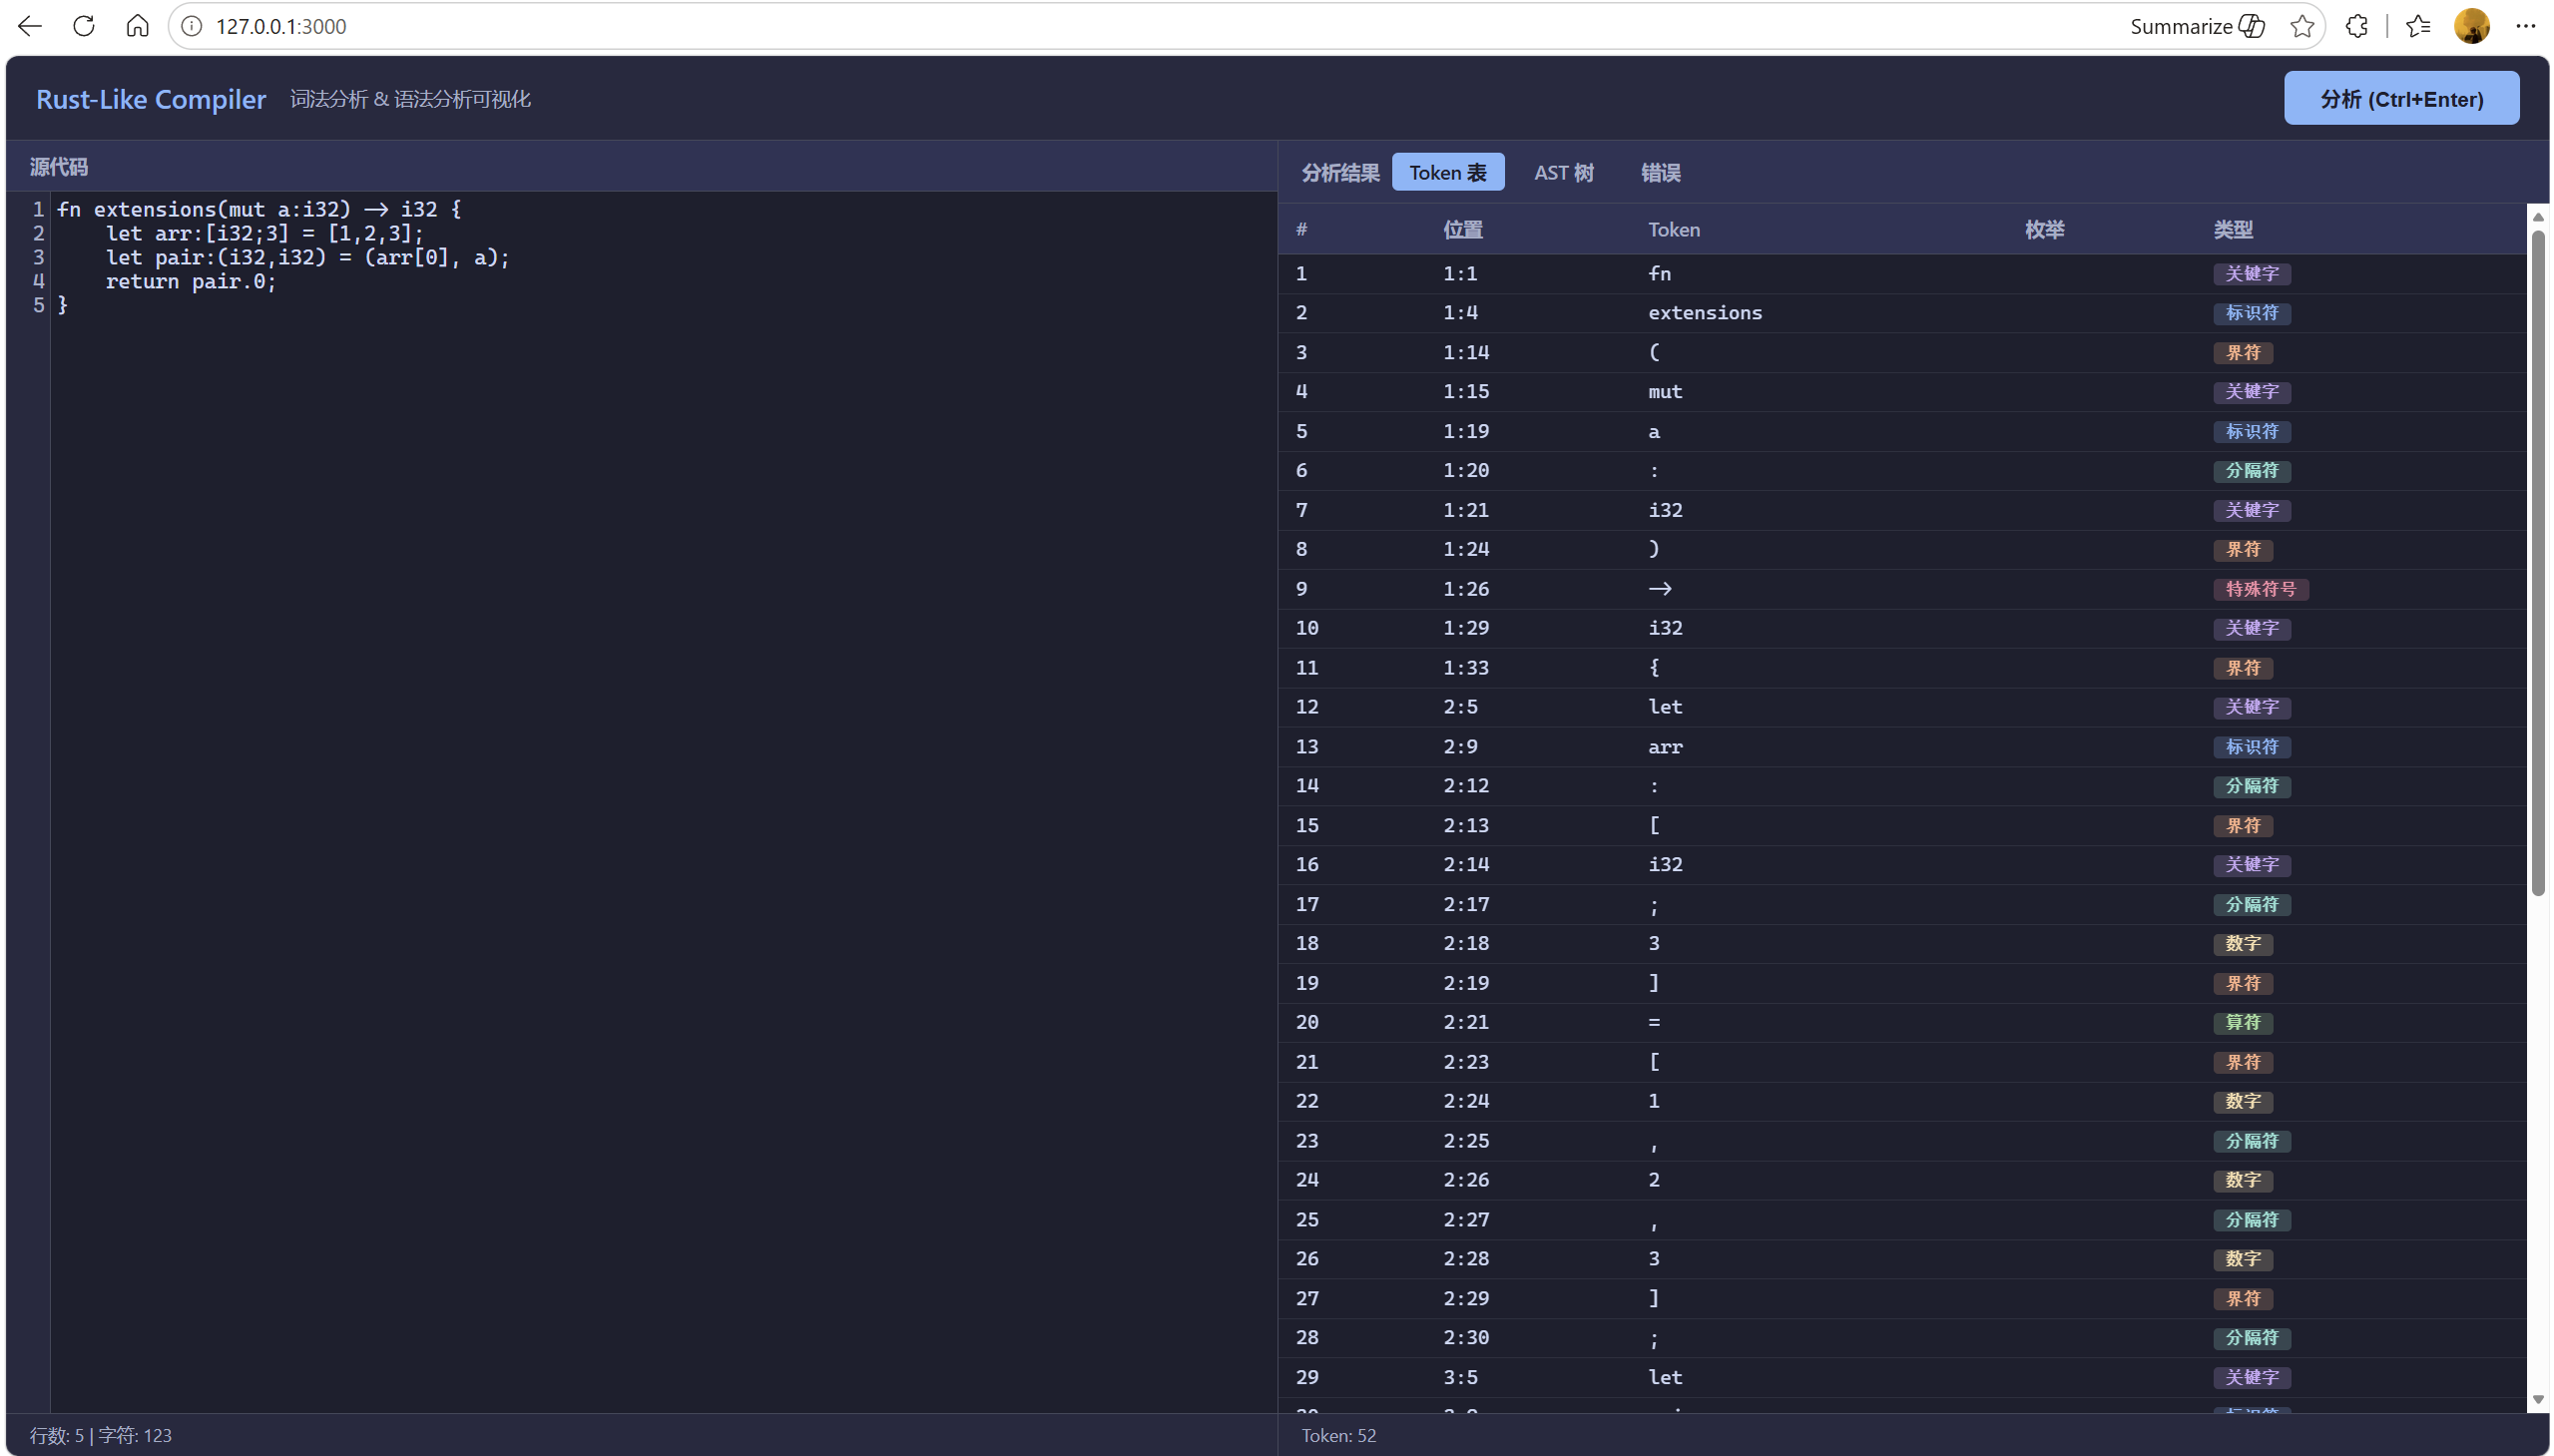
\includegraphics[width=0.8\textwidth]{figures/web_test_tokenTable.png}
    \caption{Web 页面中 token 展示设计}
    \label{fig:token-display-design}
\end{figure}

通过这种展示方式，用户可以清楚观察词法分析器如何将源代码拆分为 token。例如，输入 \texttt{if=123} 时，页面应能显示出关键字 \texttt{if}、算符 \texttt{=} 和数字 \texttt{123} 三个 token，从而验证关键字边界和 token 分割的正确性。

\subsection{AST 展示设计}

当词法分析没有错误且语法分析成功时，后端会将语法分析器生成的 AST 转换为 JSON 格式返回前端。AST 展示的目标是让用户能够观察源程序的层次化结构，例如程序由哪些函数组成，函数包含哪些参数和返回类型，函数体中有哪些语句，表达式之间具有怎样的嵌套关系。

AST 的 JSON 形式通常包含明确的 \texttt{kind} 字段。例如，顶层节点为 \texttt{Program}，函数声明节点为 \texttt{FunctionDecl}，语句节点可能为 \texttt{Let}、\texttt{Assign}、\texttt{Return}、\texttt{While} 等，表达式节点可能为 \texttt{Binary}、\texttt{Call}、\texttt{Identifier} 或 \texttt{Number} 等。通过这些节点类型，用户可以直观看到语法分析器对源程序结构的理解。

在 Web 页面中，AST 可以采用格式化 JSON 结构展示。

\begin{figure}[H]
    \centering
    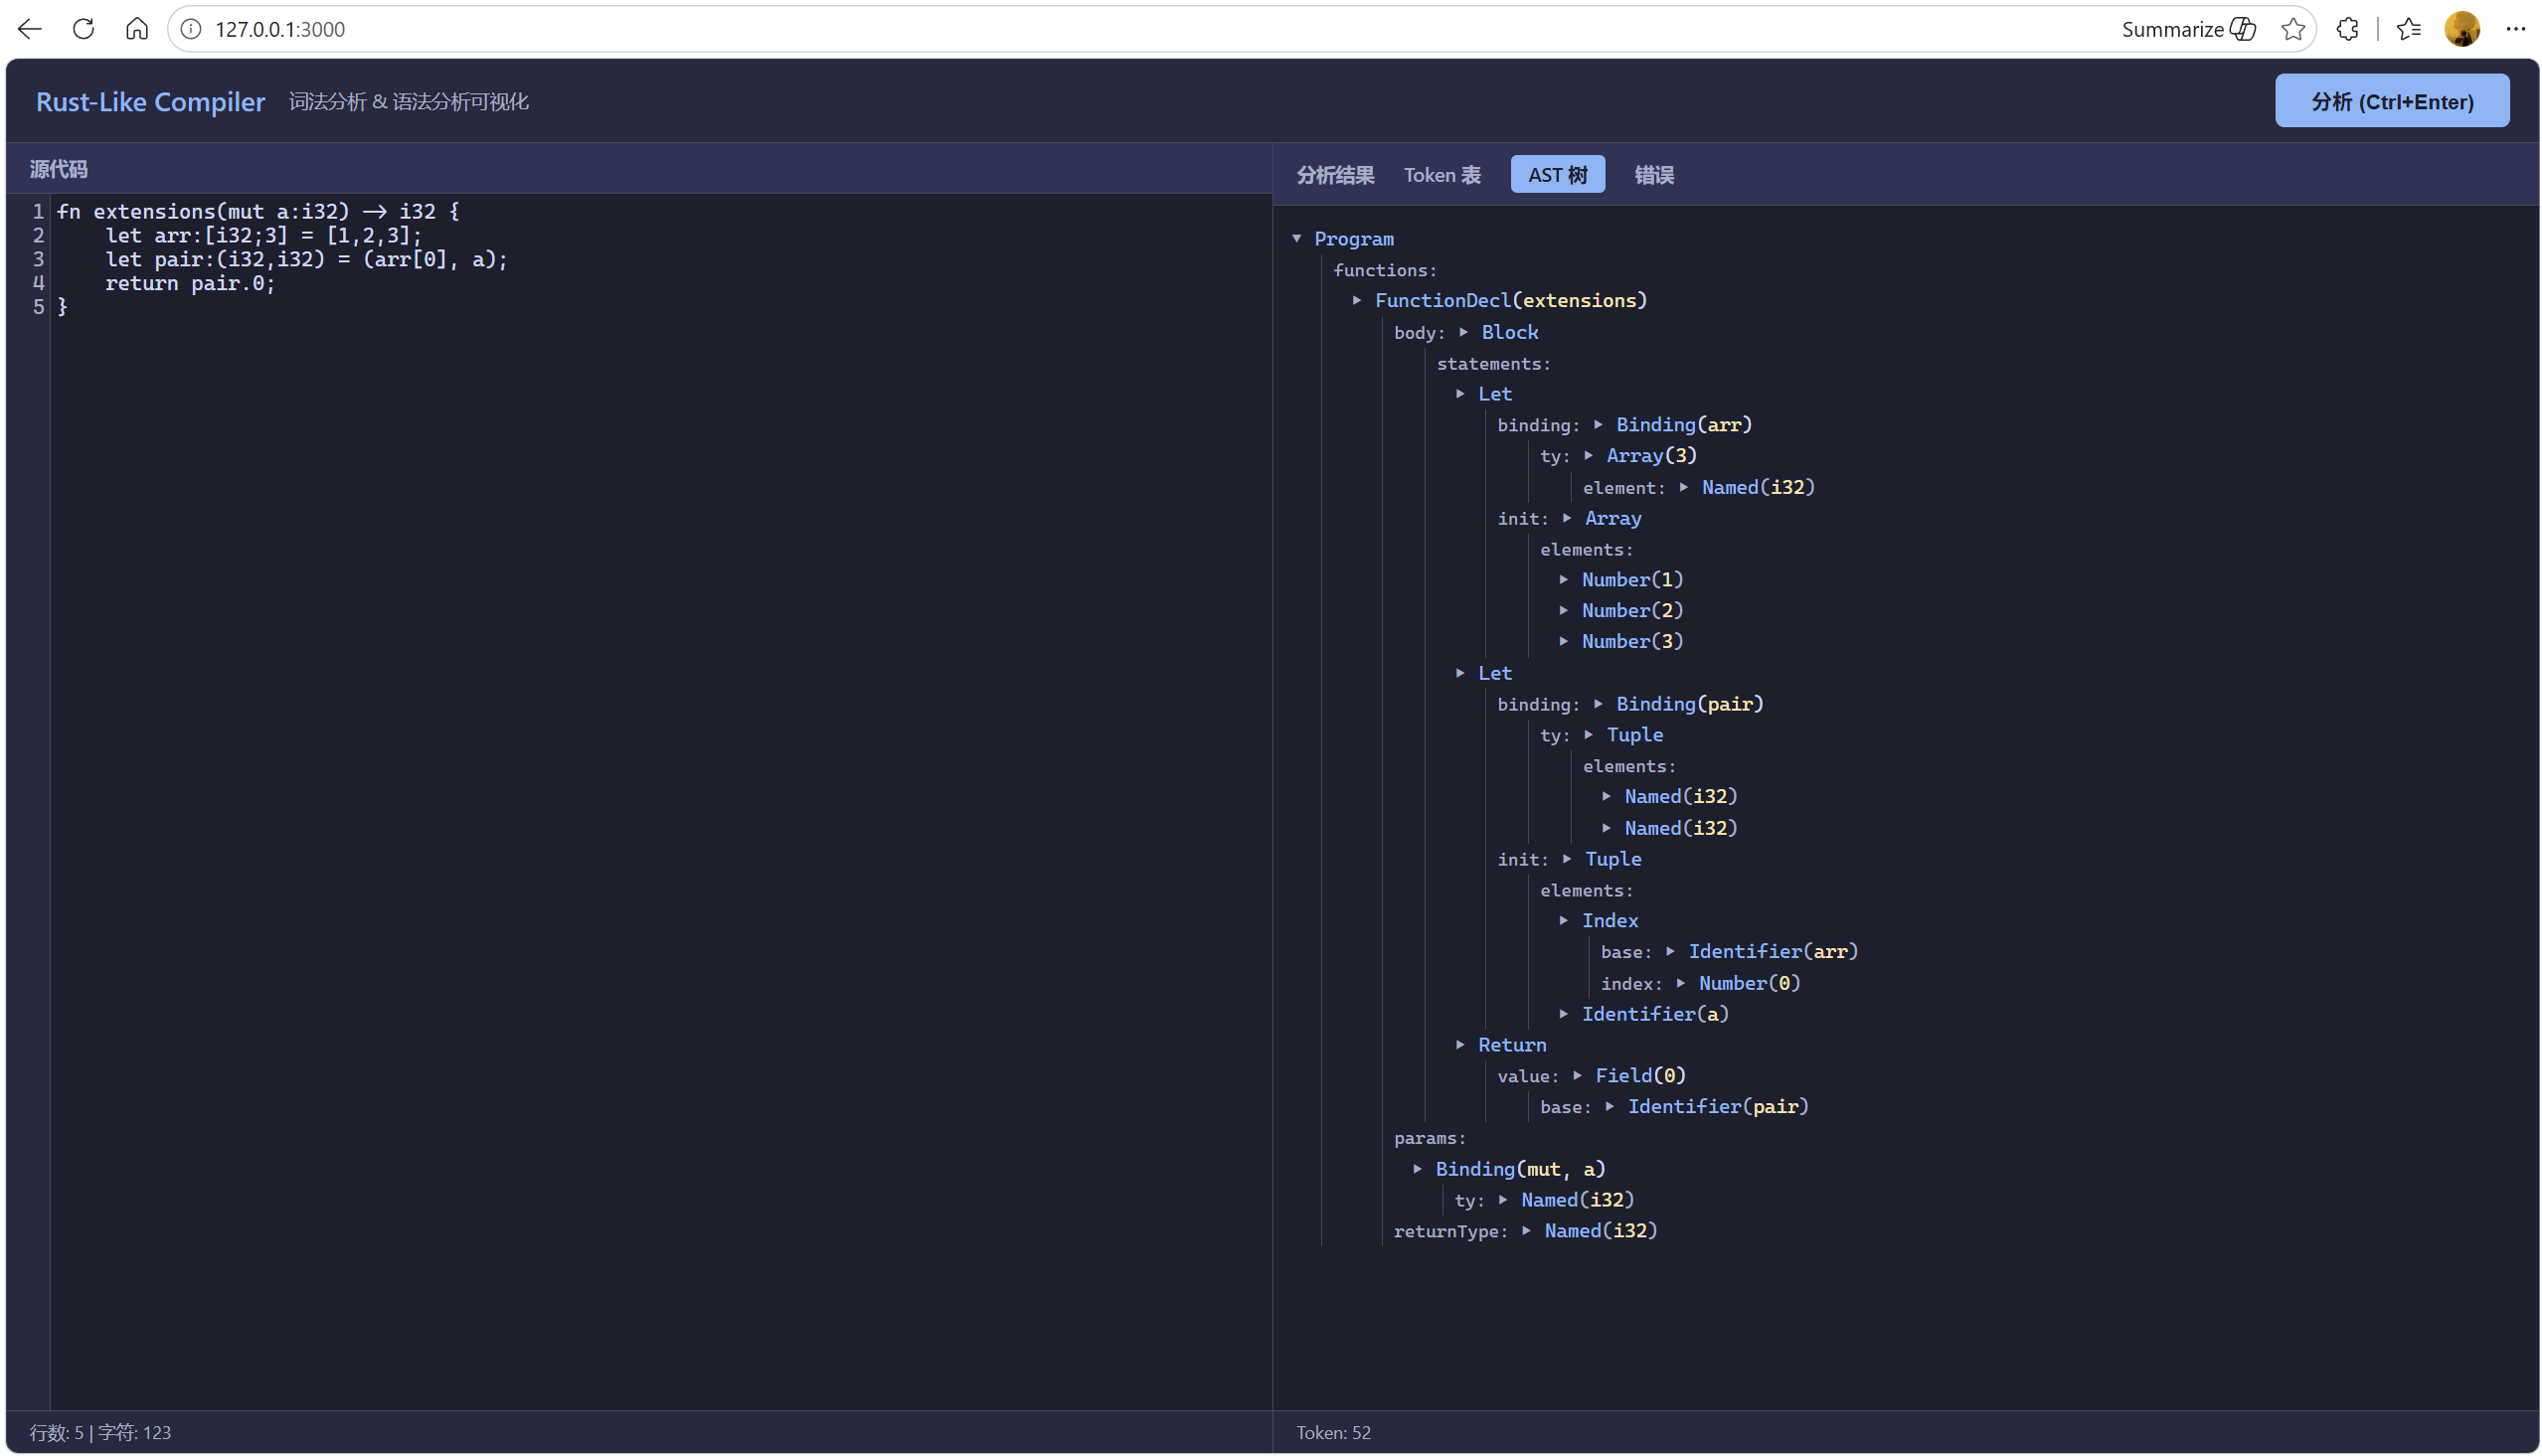
\includegraphics[width=0.8\textwidth]{figures/web_test_ast.png}
    \caption{Web 页面中 AST 展示设计}
    \label{fig:ast-display-design}
\end{figure}

AST 展示对于本项目具有重要意义。词法分析结果只能说明源程序被拆分成了哪些 token，而 AST 能进一步说明这些 token 如何组成合法的程序结构。例如，对于表达式 \texttt{a+1*2}，token 表只能显示 \texttt{a}、\texttt{+}、\texttt{1}、\texttt{*}、\texttt{2}；而 AST 可以显示乘法表达式嵌套在加法表达式右侧，从而体现表达式优先级处理的正确性。

\subsection{错误信息展示设计}

Web 系统同时展示词法错误和语法错误。二者来自不同阶段，含义也有所不同。

词法错误由词法分析器产生，主要包括无法识别的字符、未闭合块注释等问题。后端会将词法错误格式化为带有行号、列号和错误描述的字符串，并返回给前端。前端可以将这些错误集中展示在错误区域中。

\begin{figure}[H]
    \centering
    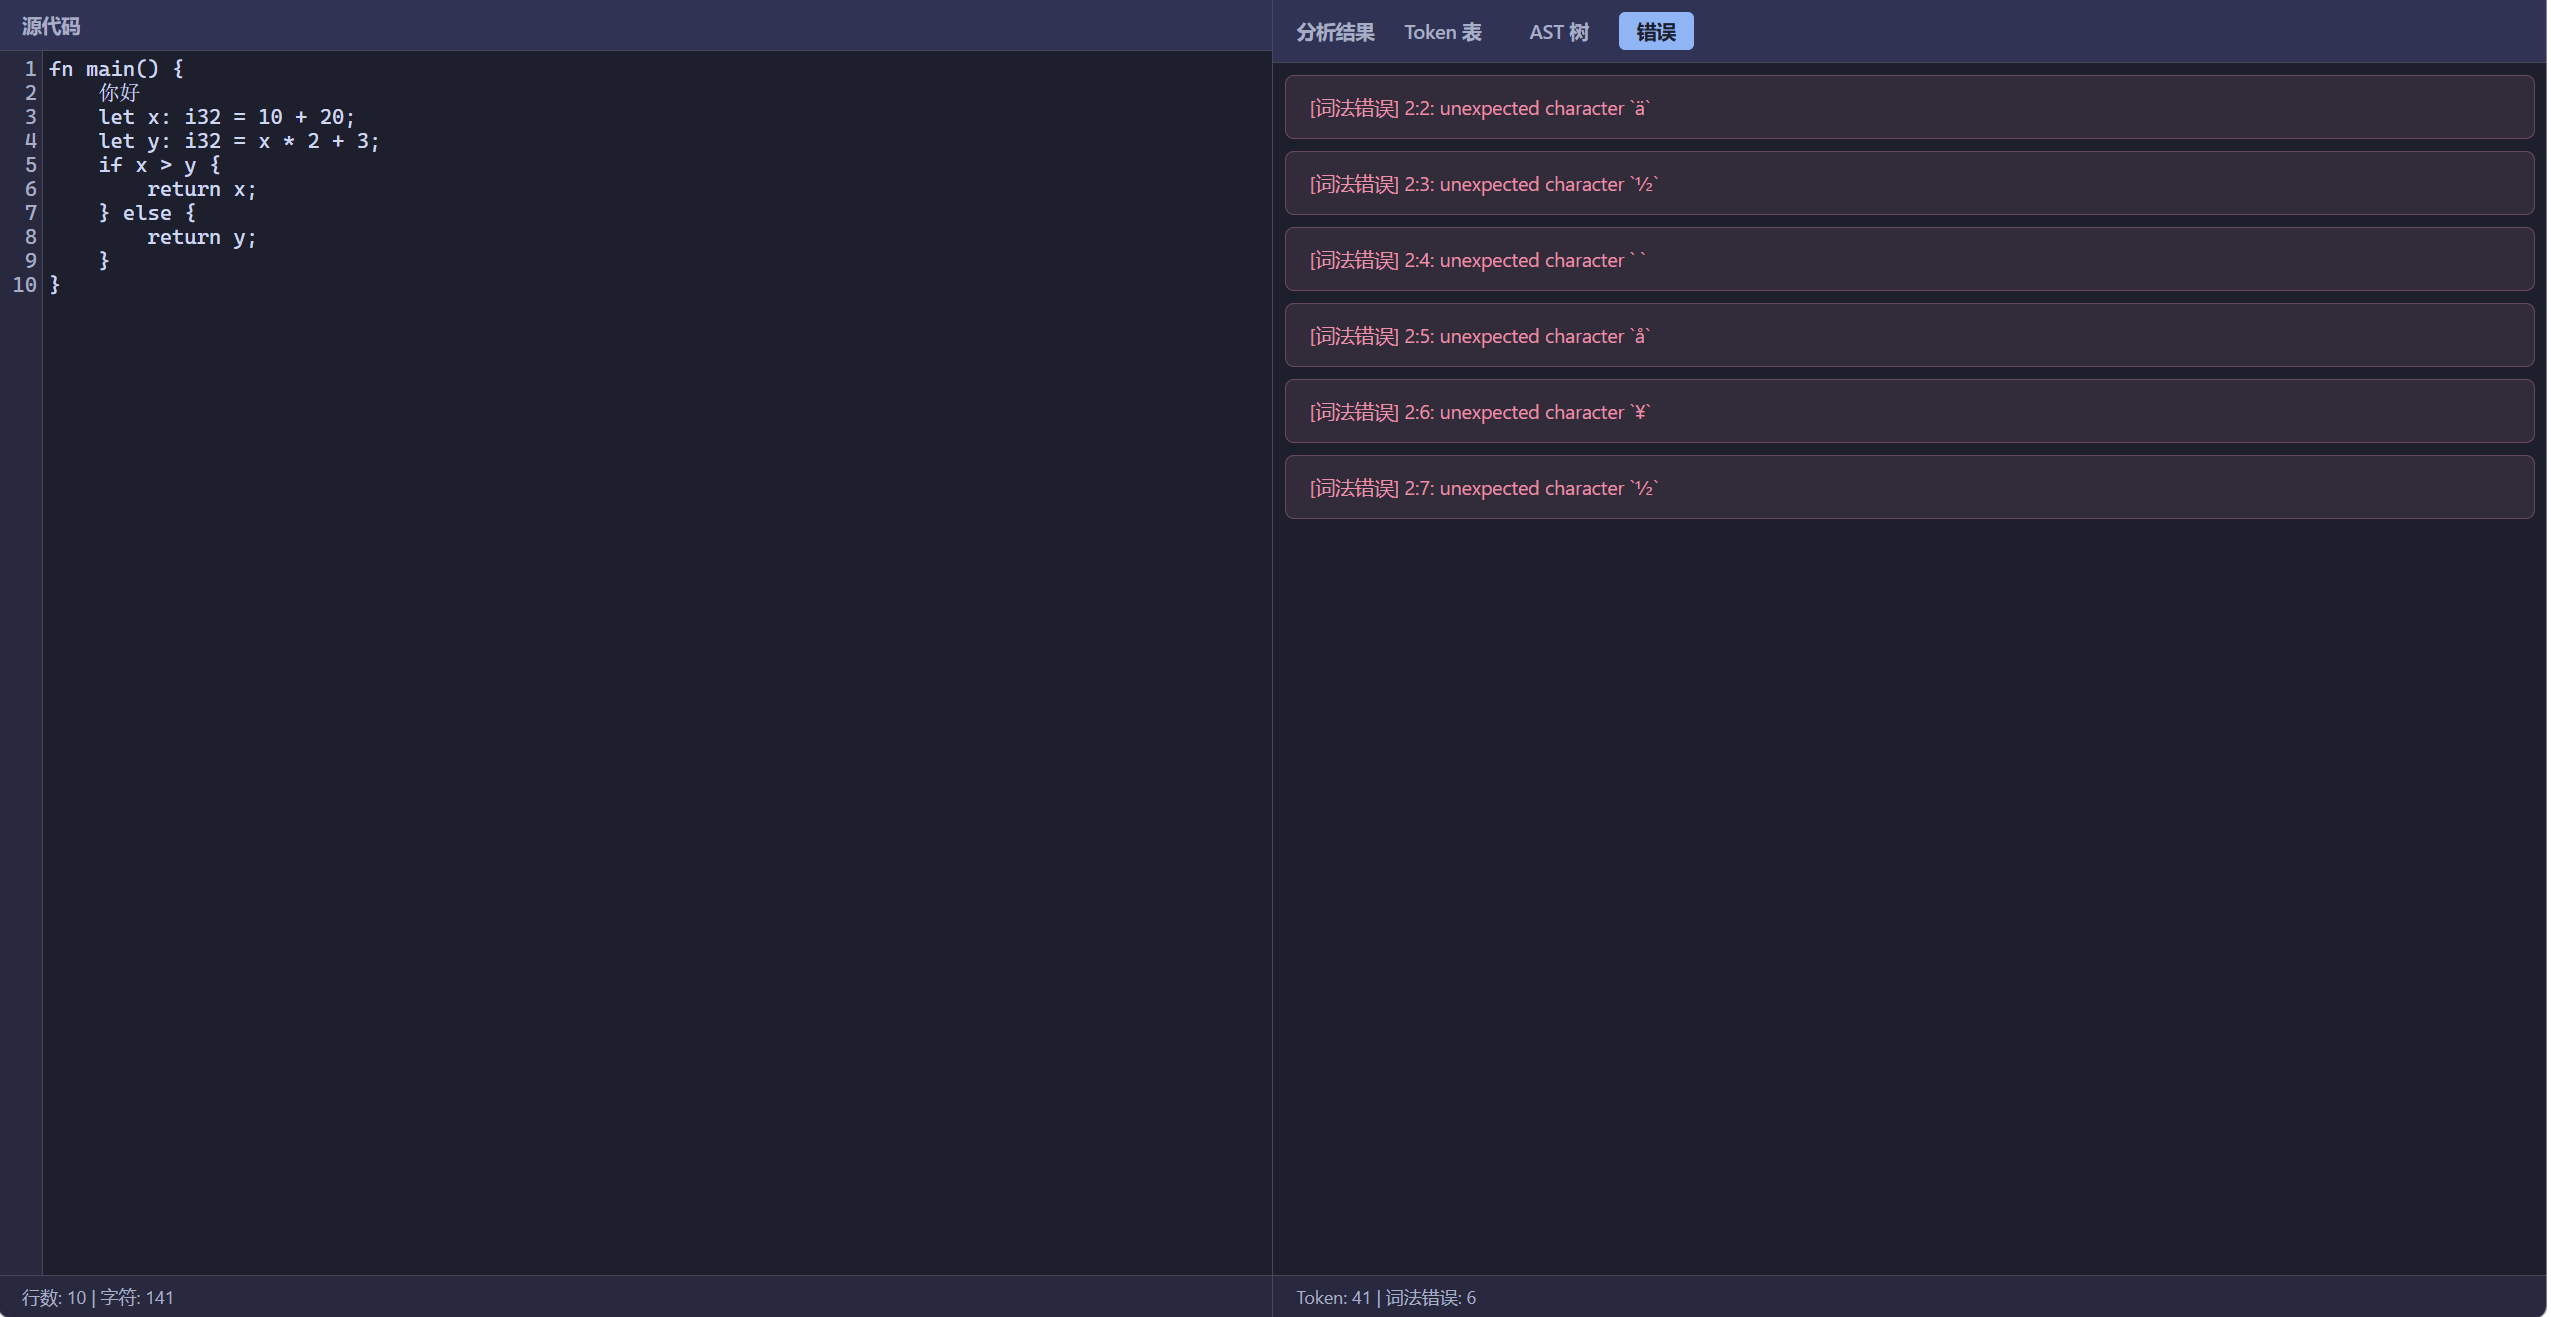
\includegraphics[width=0.8\textwidth]{figures/web_test_lexerError.png}
    \caption{Web 页面中词法错误展示设计}
    \label{fig:lexer-error-display-design}
\end{figure}

语法错误由语法分析器产生，主要包括缺少分号、缺少括号、函数声明不完整、表达式不合法、赋值左侧不可赋值等问题。由于语法分析器的错误类型中也包含位置信息，因此语法错误同样可以显示具体行列号和错误原因。

\begin{figure}[H]
    \centering
    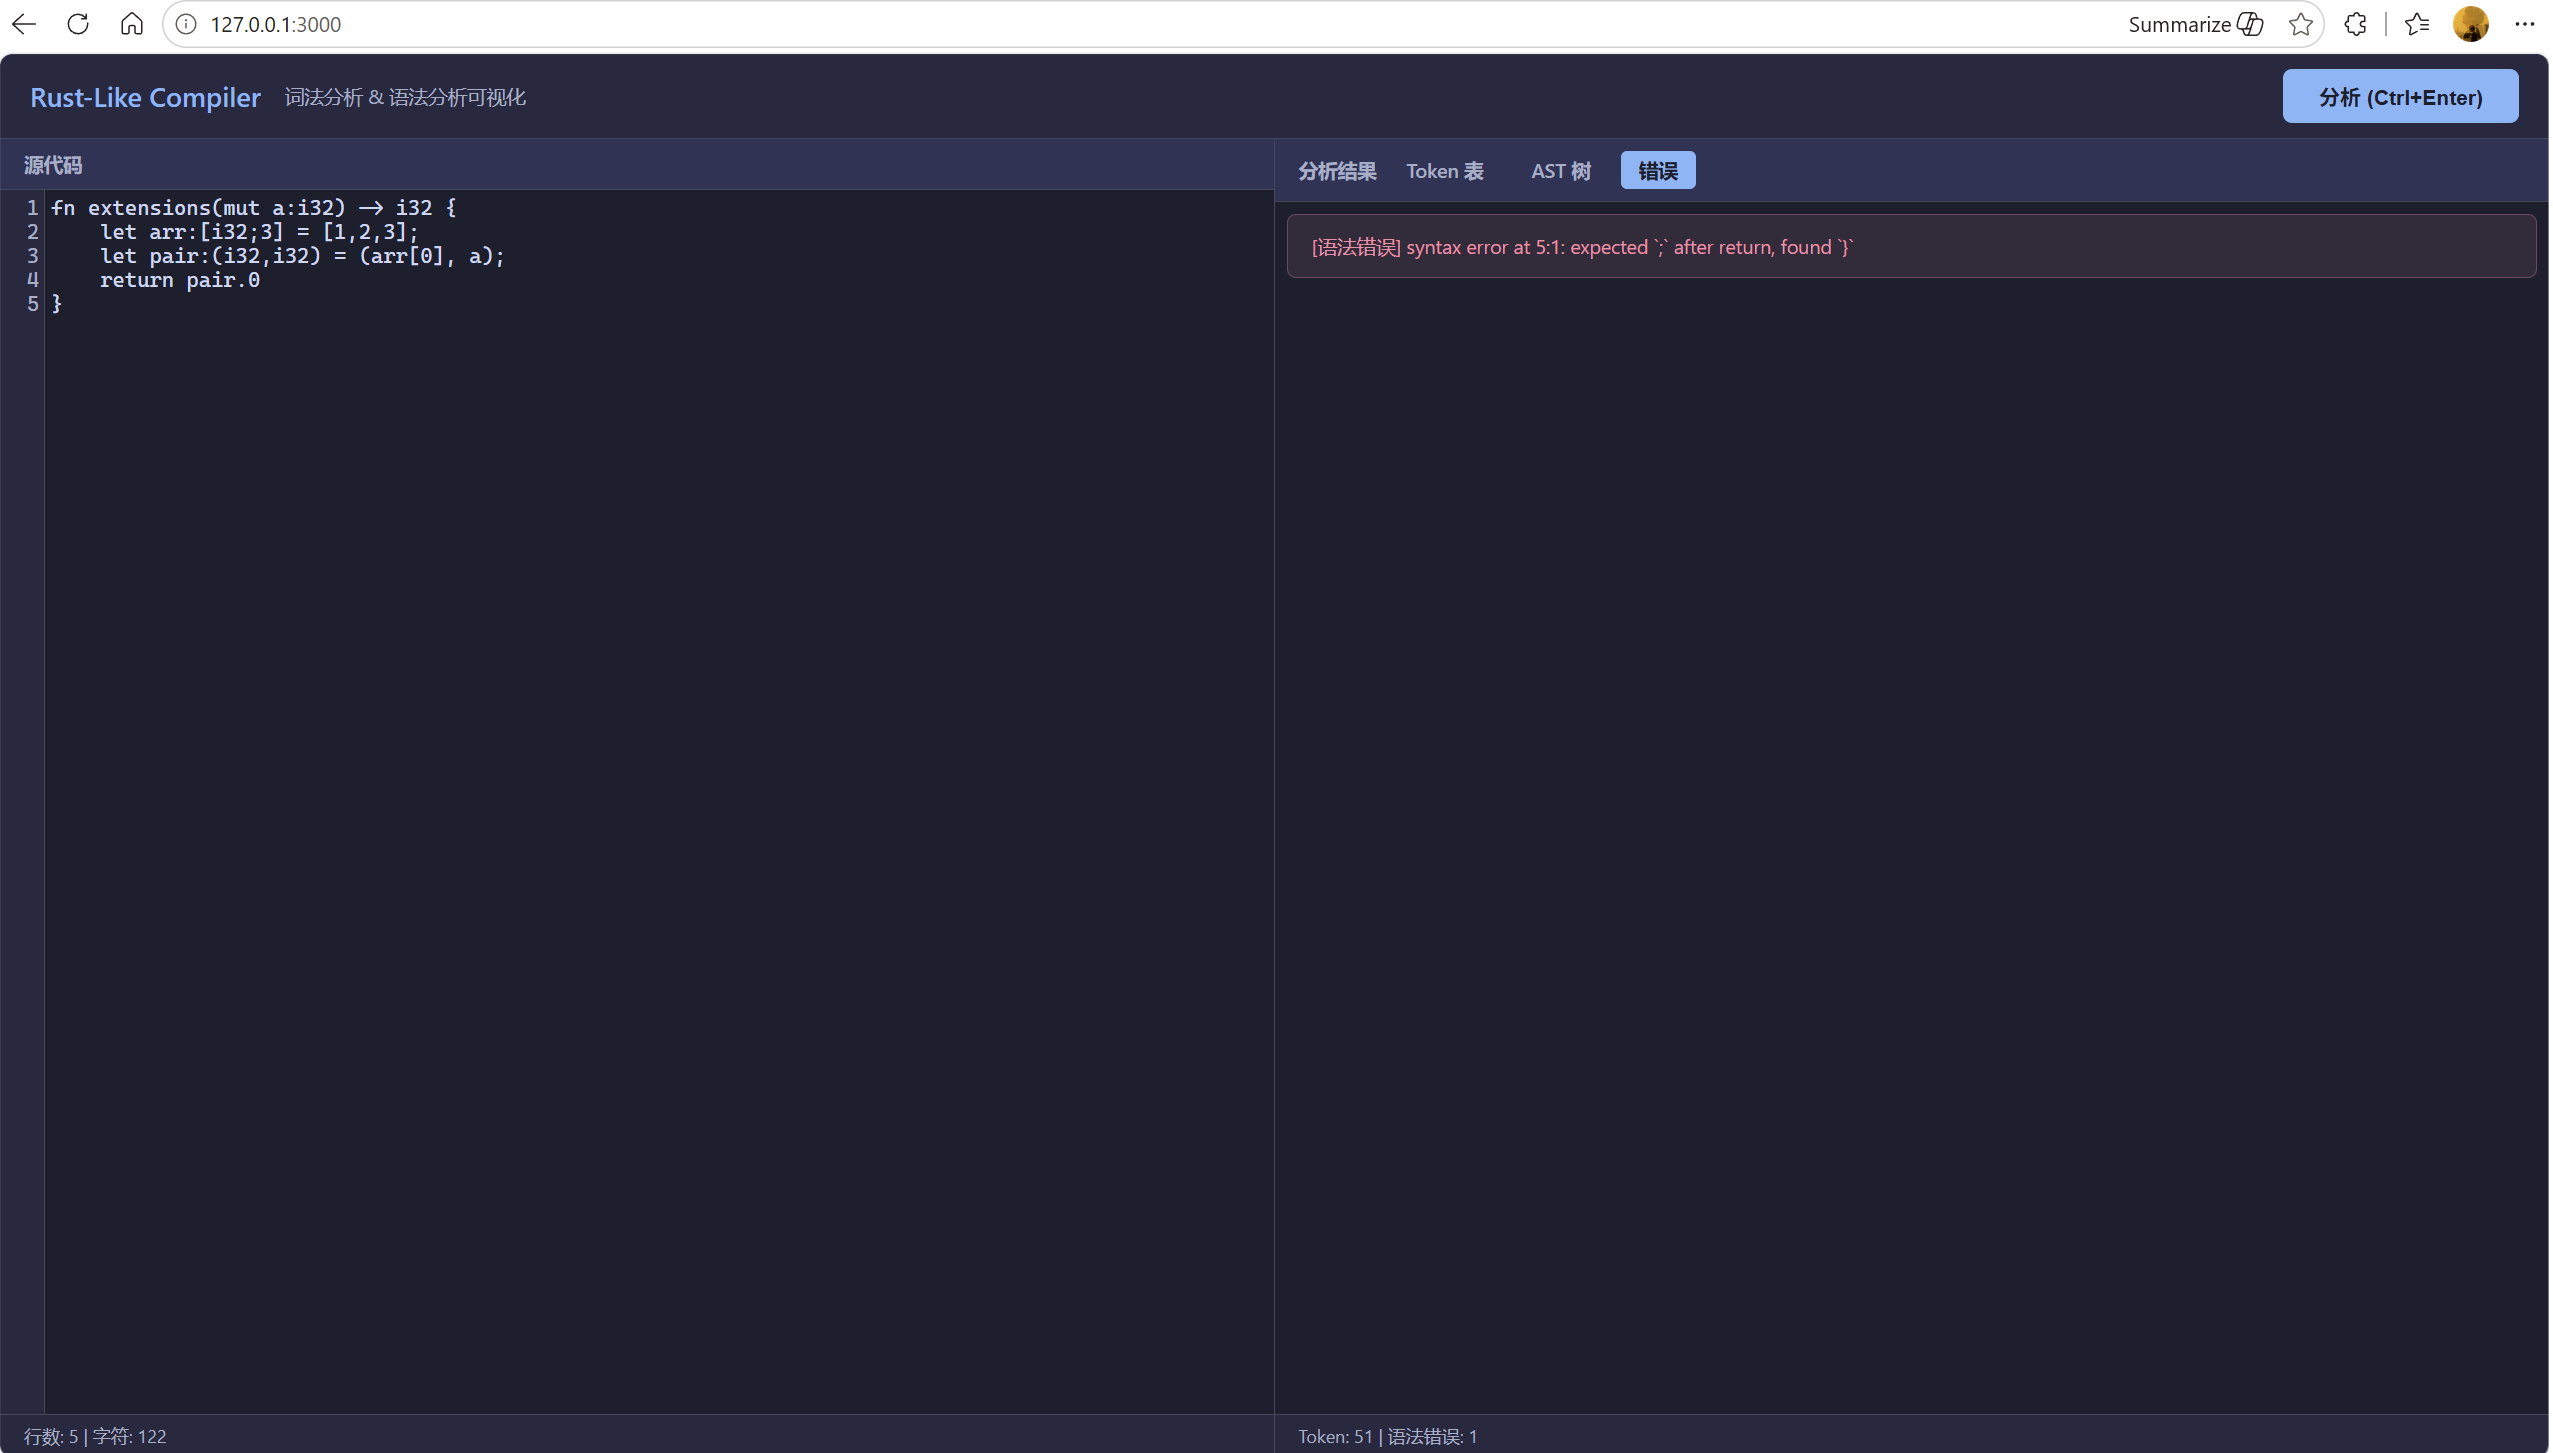
\includegraphics[width=0.85\textwidth]{figures/web_test_parserError.png}
    \caption{Web 页面中语法错误展示设计}
    \label{fig:parser-error-display-design}
\end{figure}

本系统采用了较为清晰的错误处理顺序：如果词法分析阶段已经发现错误，则后端不会继续进行语法分析。这是合理的，因为语法分析依赖 token 流的正确性；若 token 流中已经存在词法问题，继续语法分析可能产生大量连锁错误，反而干扰用户判断真正原因。

因此，Web 页面中的错误展示逻辑可以概括为：

\begin{itemize}
    \item 若存在词法错误，则展示词法错误，并不展示 AST；
    \item 若词法分析成功但语法分析失败，则展示语法错误；
    \item 若词法分析和语法分析均成功，则展示 token 表和 AST；
    \item 若没有错误，则错误区域可以为空或显示“分析成功”。
\end{itemize}

这种设计使用户能够按照编译前端的处理顺序理解错误来源：先检查字符级和 token 级问题，再检查语法结构问题。

\subsection{Web 可视化系统的作用}

Web 可视化系统在本项目中主要发挥两个方面的作用。

第一，它提高了系统的可操作性。用户不需要分别运行词法分析器和语法分析器命令，也不需要手动查看 JSON 文件，只需要在浏览器中输入代码即可获得完整分析结果。

第二，它验证了模块复用能力。Web 服务本身并没有重新实现词法分析和语法分析，而是直接调用 \texttt{Easy\_Lexer} 和 \texttt{Easy\_Parser}。这说明项目底层模块具有较好的独立性，可以被命令行程序、测试程序和 Web 服务共同复用。
\section{实验测试与结果分析}

\subsection{测试环境}

\begin{table}[H]
    \centering
    \caption{测试环境}
    \begin{tabularx}{\textwidth}{c|Y}
        \toprule
        项目 & 内容 \\
        \midrule
        操作系统 & Windows \\
        编程语言 & Rust \\
        构建工具 & Cargo \\
        浏览器 & Edge / Chrome \\
        测试方式 & 单元测试、集成测试、命令行测试、Web 页面测试 \\
        \bottomrule
    \end{tabularx}
\end{table}

\subsection{词法分析测试}

代码中为词法分析器设计了多个单元测试，用于验证关键词法功能是否符合预期。这些测试不仅验证了基本 token 识别，也覆盖了课程中特别强调的边界情况。

\subsubsection{关键字后缀测试}

测试 \texttt{keyword\_suffix\_stays\_identifier} 用于验证 \texttt{if123} 不会被错误拆分，而是作为一个完整标识符识别。

\begin{lstlisting}[language=Rust,caption={关键字后缀测试}]
#[test]
fn keyword_suffix_stays_identifier() {
    let result = lex("if123");
    assert!(result.errors.is_empty());
    assert_eq!(result.tokens.len(), 1);
    assert_eq!(result.tokens[0].kind, TokenKind::Identifier);
    assert_eq!(result.tokens[0].lexeme, "if123");
}
\end{lstlisting}

该测试说明词法分析器采用的是“先完整读取标识符，再判断是否为关键字”的策略，而不是简单的关键字前缀匹配。

\subsubsection{关键字、赋值号和整数拆分测试}

测试 \texttt{keyword\_operator\_number\_are\_split} 用于验证 \texttt{if=123} 能够被正确拆分为关键字、赋值号和数字。

\begin{lstlisting}[language=Rust,caption={关键字、赋值号和整数拆分测试}]
#[test]
fn keyword_operator_number_are_split() {
    let result = lex("if=123");
    assert!(result.errors.is_empty());
    assert_eq!(
        result
            .tokens
            .iter()
            .map(|token| &token.kind)
            .collect::<Vec<_>>(),
        vec![
            &TokenKind::Keyword(Keyword::If),
            &TokenKind::Assign,
            &TokenKind::Number,
        ]
    );
}
\end{lstlisting}

该测试对应课程要求中的特殊样例，验证了词法分析器在关键字边界和不同 token 分界上的正确性。

\subsubsection{注释跳过测试}

测试 \texttt{comments\_are\_skipped} 用于验证块注释和单行注释不会生成 token。

\begin{lstlisting}[language=Rust,caption={注释跳过测试}]
#[test]
fn comments_are_skipped() {
    let result = lex("let /* block */ mut // line\n a");
    assert!(result.errors.is_empty());
    assert_eq!(
        result
            .tokens
            .iter()
            .map(|token| token.lexeme.as_str())
            .collect::<Vec<_>>(),
        vec!["let", "mut", "a"]
    );
}
\end{lstlisting}

该测试表明，注释内容被正确忽略，最终输出中只保留有效 token。

\subsubsection{最长匹配测试}

测试 \texttt{longest\_match\_tokens\_win} 用于验证复合 token 的优先识别。

\begin{lstlisting}[language=Rust,caption={最长匹配测试}]
#[test]
fn longest_match_tokens_win() {
    let result = lex("-> == >= <= != .. .");
    assert!(result.errors.is_empty());
    assert_eq!(
        result
            .tokens
            .iter()
            .map(|token| &token.kind)
            .collect::<Vec<_>>(),
        vec![
            &TokenKind::Arrow,
            &TokenKind::EqualEqual,
            &TokenKind::GreaterEqual,
            &TokenKind::LessEqual,
            &TokenKind::NotEqual,
            &TokenKind::DotDot,
            &TokenKind::Dot,
        ]
    );
}
\end{lstlisting}

该测试说明 \texttt{->}、\texttt{==}、\texttt{>=}、\texttt{<=}、\texttt{!=} 和 \texttt{..} 都会优先于其单字符前缀被识别，从而满足词法分析中的最长匹配原则。

\subsubsection{未闭合块注释测试}

测试 \texttt{unterminated\_block\_comment\_reports\_error} 用于验证未闭合块注释能够被正确报告为词法错误。

\begin{lstlisting}[language=Rust,caption={未闭合块注释测试}]
#[test]
fn unterminated_block_comment_reports_error() {
    let result = lex("/* oops");
    assert!(result.tokens.is_empty());
    assert_eq!(result.errors.len(), 1);
    assert!(result.errors[0].message.contains("unterminated"));
}
\end{lstlisting}

该测试说明词法分析器能够发现块注释缺少结束符的问题，并将其记录在错误列表中。

\subsubsection{集成测试}
除了单元测试之外，还设计了集成测试，验证词法分析器和语法分析器能够正确处理实际源代码文件，并将结果输出为 txt 文件。通过与预期结果文件进行比对，可以验证系统的整体正确性。
输入的测试源代码位于 \texttt{Easy\_lexer} 文件夹的 tests 目录下，命名为 \texttt{input.rs}；输出的 txt 结果文件位于 output 目录下，Lexer 和 Parser 均可调用测试模块对实现效果进行测试。下面是集成测试的示例代码，代码中覆盖了已经实现的所有依赖功能。

\begin{lstlisting}[language=Rust,caption={集成测试}]
#[test]
fn helper() {
}

fn compute(mut base:i32, limit:i32) -> i32 {
    ;
    let plain;
    let typed:i32;
    let mut value:i32=base+1*2;
    let arr:[i32;3]=[1,2,3];
    let mut pair:(i32,i32)=(arr[0], value);
    let unit:()=();
    let ref_value:&i32=&value;
    let mut ref_mut:&mut i32=&mut value;

    plain=0;
    typed=(plain+value)/2;
    pair.0=typed;
    *ref_mut=pair.0-1;
    arr[1];
    pair.1;
    helper();
    helper(value, arr[2]);
    -value;
    &value;
    &mut value;
    *ref_mut;
    { let t:i32=1; t };

    if value>=limit {
        value=value-1;
    } else if value!=0 {
        value=value+1;
    } else {
        return;
    }

    while value>0 {
        if value==2 {
            break;
        }
        value=value-1;
    }

    for mut i in 0..limit {
        if i<=1 {
            continue;
        }
    }

    for item in arr {
        item;
    }

    loop {
        break;
    }

    let loop_value=loop {
        break 7;
    };
    let chosen=if value<limit { value } else { limit };

    return chosen;
}
#
\end{lstlisting}

\subsubsection{词法分析结果}
词法分析的测试结果如下：

\begin{figure}[H]
    \centering
    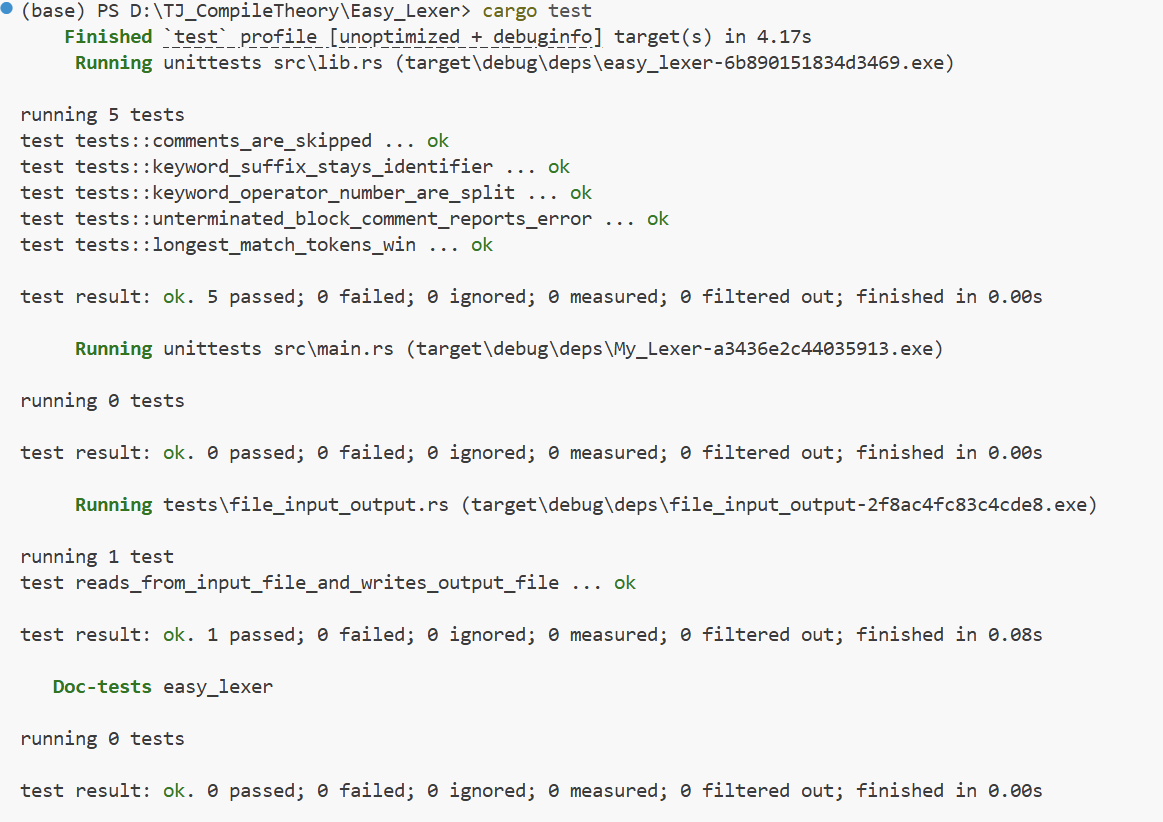
\includegraphics[width=0.85\textwidth]{figures/lexer_test.png}
    \caption{词法分析结果截图}
\end{figure}

\subsection{语法分析测试}

代码中为语法分析器设计了多个测试用例，用于验证最低语法要求、扩展语法、错误处理和结束符处理。

\subsubsection{最低语法规则测试}

测试 \texttt{parses\_minimum\_required\_grammar} 覆盖了课程要求中的核心语法结构：

\begin{lstlisting}[language=Rust,caption={最低语法规则测试示例}]
#[test]
fn parses_minimum_required_grammar() {
    parse_ok(
        r#"
        fn base(mut a:i32) -> i32 {
            ;
            let mut b:i32;
            let c=1;
            a=a+1*2;
            if a>0 {
                foo(a, c);
            }
            while a!=0 {
                a=a-1;
            }
            return a;
        }

        fn foo(x:i32, y:i32) {
            x+y;
        }
        "#,
    );
}
\end{lstlisting}

该测试包含函数声明、参数、返回类型、空语句、变量声明、变量声明赋值、赋值语句、表达式、if 结构、while 循环、函数调用和返回语句，能够较好验证课程强制要求是否被覆盖。

\subsubsection{扩展语法测试}

测试 \texttt{parses\_extended\_constructs} 用于验证扩展语法：

\begin{lstlisting}[language=Rust,caption={扩展语法测试示例}]
#[test]
fn parses_extended_constructs() {
    let ast = parse_ok(
        r#"
        fn extra(mut a:i32) -> i32 {
            let mut arr:[i32;3]=[1,2,3];
            let mut pair:(i32,i32)=(arr[0], a);
            let r:&mut i32=&mut a;
            let v={
                let t=pair.0;
                if t>0 { t } else { 0 }
            };
            for mut i in 0..a {
                if i==2 { continue; }
            }
            let b=loop {
                break v;
            };
            return b;
        }
        "#,
    );
    serde_json::to_string_pretty(&ast).unwrap();
}
\end{lstlisting}

该测试覆盖数组类型和数组字面量、元组类型和元组字段访问、可变引用、块表达式、if 表达式、for 循环、区间表达式、continue、loop 表达式和 break 表达式等内容。测试中还调用 \texttt{serde\_json::to\_string\_pretty}，验证 AST 能够正确序列化为 JSON。

\subsubsection{赋值目标错误测试}

测试 \texttt{reports\_assignment\_target\_errors} 用于验证非法赋值目标能够被识别：

\begin{lstlisting}[language=Rust,caption={赋值目标错误测试}]
#[test]
fn reports_assignment_target_errors() {
    let result = lex(r#"
        fn bad() {
            1=2;
        }
        "#);
    let error = parse_tokens(&result.tokens).unwrap_err();
    assert!(error.message.contains("not assignable"));
}
\end{lstlisting}

该测试说明解析器并不是简单地接受所有“表达式 = 表达式”的形式，而是会检查左侧表达式是否满足可赋值条件。

\subsubsection{结束符测试}

测试 \texttt{accepts\_end\_marker} 用于验证课程要求中的结束符 \texttt{\#} 可以被接受：

\begin{lstlisting}[language=Rust,caption={结束符测试}]
#[test]
fn accepts_end_marker() {
    parse_ok(
        r#"
        fn done() {
            return;
        }
        #
        "#,
    );
}
\end{lstlisting}

该测试对应 \texttt{parse\_program} 中对 \texttt{EndMarker} 的处理逻辑。

\subsubsection{语法分析结果}
语法分析的测试结果如下：

\begin{figure}[H]
    \centering
    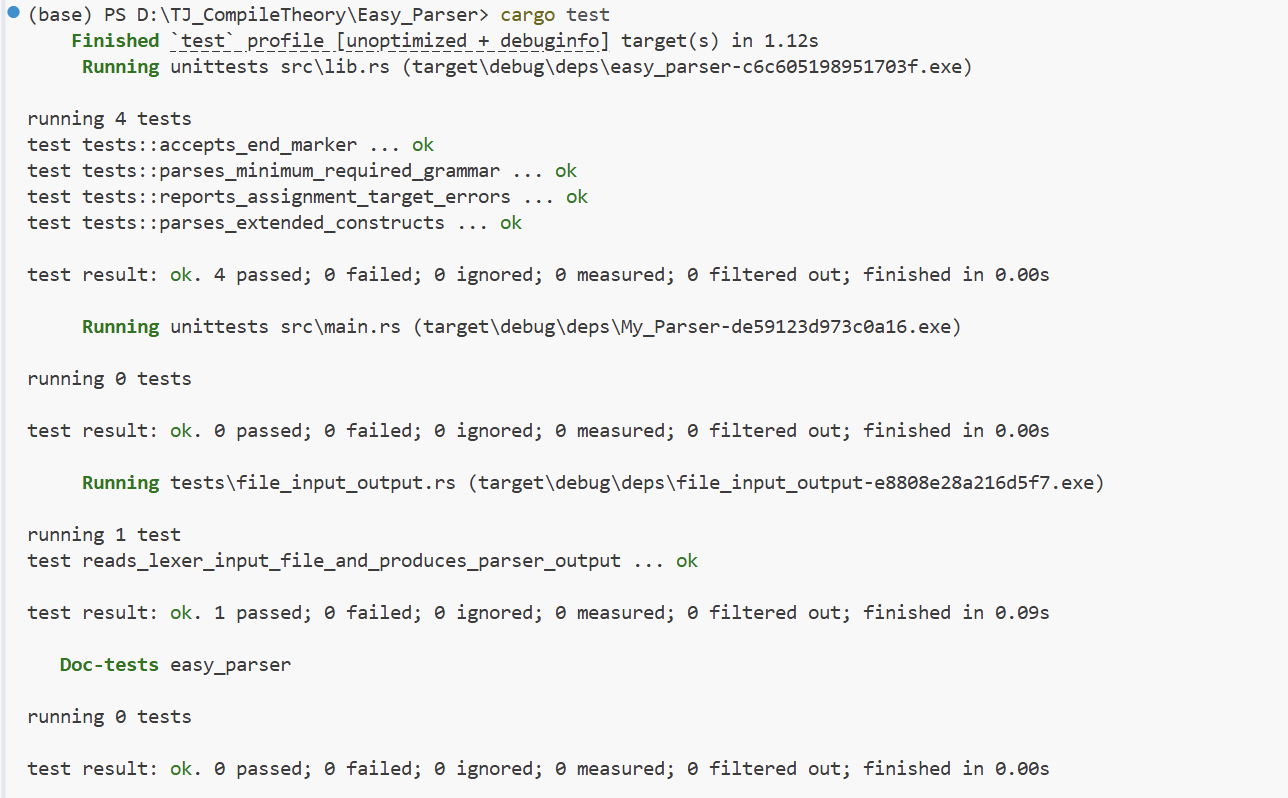
\includegraphics[width=0.85\textwidth]{figures/parser_test.png}
    \caption{语法分析结果截图}
\end{figure}

\section{改进方向}

当前项目已经完成了类 Rust 语言的词法分析和语法分析主体，能够将源程序转换为 token 序列，并进一步构造抽象语法树。但从完整编译器前端的角度来看，当前系统仍主要停留在词法和语法结构识别阶段，尚未形成完整的语义分析能力。后续可以在现有 AST 基础上，从符号表、类型检查和可变性检查三个方面继续完善。

\subsection{增加符号表}

当前语法分析器能够识别变量声明、函数参数、赋值语句和表达式等结构，但尚未系统记录程序中已经声明过的变量、函数及其作用域信息。因此，后续可以增加符号表结构，用于保存变量名、类型、是否可变、声明位置、所属作用域等信息。

符号表可以随着语法树遍历过程逐步建立。例如，在进入一个函数体或语句块时创建新的作用域，在遇到变量声明或函数参数时将其加入当前作用域，在离开语句块时销毁对应作用域。通过这种方式，可以支持对局部变量、函数参数以及嵌套语句块中变量可见性的管理。

引入符号表后，系统可以进一步检查以下问题：

\begin{itemize}
    \item 变量在使用前是否已经声明；
    \item 同一作用域中是否存在重复声明；
    \item 内层作用域变量是否正确覆盖外层变量；
    \item 赋值语句或表达式中引用的标识符是否能够在当前作用域中找到。
\end{itemize}

因此，符号表是后续语义分析的基础。没有符号表，语法分析器只能判断程序结构是否符合文法；有了符号表后，系统才能进一步判断程序中名称使用是否合理。

\subsection{实现基础类型检查}

在符号表基础上，后续可以进一步实现基础类型检查。当前项目虽然在 AST 中已经能够表示 \texttt{i32}、数组、元组、引用等类型结构，但这些类型信息主要用于语法结构展示，并没有系统参与语义判断。例如，解析器可以识别 \texttt{let a:i32;}、\texttt{let arr:[i32;3];}、\texttt{let pair:(i32,i32);} 等声明，但还不会完整检查后续赋值或表达式计算是否符合类型规则。


例如，对于函数：

\begin{lstlisting}[language=Rust,caption={返回类型检查示例}]
fn f() -> i32 {
    return;
}
\end{lstlisting}

语法上它可能可以被解析，但从语义上看，函数声明返回 \texttt{i32}，而 \texttt{return;} 没有返回表达式，因此应当报告返回类型不一致错误。类似地，若将数组赋值给 \texttt{i32} 变量，也应当被类型检查阶段识别为错误。

因此，类型检查可以使系统从“能否解析程序结构”进一步提升到“能否判断程序结构是否具有合理含义”。

\subsection{实现可变性检查}

Rust 语言的一个重要特点是变量默认不可变，只有显式声明为 \texttt{mut} 的变量才允许被重新赋值。当前项目在词法和语法层面已经能够识别 \texttt{mut} 关键字，并在 AST 的 \texttt{Binding} 节点中记录变量是否可变，但尚未完整检查后续是否存在对不可变变量重新赋值的情况。

后续可以在符号表中为每个变量记录其可变性属性。当语义分析器遇到赋值语句时，先根据赋值左侧的标识符在符号表中查找对应变量，再判断该变量是否被声明为 \texttt{mut}。如果变量没有 \texttt{mut} 标记，却出现在赋值语句左侧，则应当报告不可变变量赋值错误。

可变性检查不仅可以应用于普通变量，也可以进一步扩展到解引用赋值、数组元素赋值和元组字段赋值等情况。例如，\texttt{arr[0] = 1;} 是否合法，既取决于 \texttt{arr} 是否可变，也取决于数组类型本身是否允许该操作。因此，可变性检查需要和符号表、类型检查结合起来实现。

综上，增加可变性检查能够更好体现类 Rust 语言的特点，也能使项目从单纯的语法分析进一步接近真实 Rust 编译器前端中的语义约束处理。

\section{总结与展望}

本项目完成了词法分析器、语法分析器和 Web 可视化展示页面，
能够识别课程要求中的主要词法单元，并覆盖最低要求中的核心语法规则。
同时，项目还实现了部分扩展语法，如 \texttt{else if}、\texttt{for}、\texttt{loop}、引用、数组和元组等。

从整体完成度来看，项目已经具备课程演示所需的基本形态。
不过，当前系统仍以词法分析和语法分析为主，尚未实现完整语义分析。
未来可以从符号表、类型检查、可变性检查、返回值检查和错误恢复等方面继续完善。

\newpage

\begin{thebibliography}{99}

\bibitem{dragonbook}
Alfred V. Aho, Monica S. Lam, Ravi Sethi, Jeffrey D. Ullman.
\newblock \textit{Compilers: Principles, Techniques, and Tools}.
\newblock Pearson, 2nd Edition, 2006.

\bibitem{rustbook}
Steve Klabnik, Carol Nichols.
\newblock \textit{The Rust Programming Language}.
\newblock No Starch Press, 2019.

\bibitem{rustreference}
The Rust Project Developers.
\newblock \textit{The Rust Reference}.
\newblock \url{https://doc.rust-lang.org/reference/}

\bibitem{craftinginterpreters}
Robert Nystrom.
\newblock \textit{Crafting Interpreters}.
\newblock Genever Benning, 2021.

\bibitem{courseppt}
同济大学编译原理课程组.
\newblock \textit{【Rust版】大作业1：词法和语法分析工具设计与实现v5.0}.
\newblock 课程资料.

\end{thebibliography}

\end{document}